%%%%%%%%%%%%%%%%%%%%%%%%%%%%%%%%%%%%%%%%%
% Journal Article
% LaTeX Template
% Version 2.0 (February 7, 2023)
%
% This template originates from:
% https://www.LaTeXTemplates.com
%
% Author:
% Vel (vel@latextemplates.com)
%
% License:
% CC BY-NC-SA 4.0 (https://creativecommons.org/licenses/by-nc-sa/4.0/)
%
% NOTE: The bibliography needs to be compiled using the biber engine.
%
%%%%%%%%%%%%%%%%%%%%%%%%%%%%%%%%%%%%%%%%%

%----------------------------------------------------------------------------------------
%	PACKAGES AND OTHER DOCUMENT CONFIGURATIONS
%----------------------------------------------------------------------------------------

\documentclass[
	a4paper, % Paper size, use either a4paper or letterpaper
	10pt, % Default font size, can also use 11pt or 12pt, although this is not recommended
	unnumberedsections, % Comment to enable section numbering
	twoside, % Two side traditional mode where headers and footers change between odd and even pages, comment this option to make them fixed
]{LTJournalArticle}

\addbibresource{sample.bib} % BibLaTeX bibliography file

%\runninghead{Shortened Running Article Title} % A shortened article title to appear in the running head, leave this command empty for no running head

\footertext{\textit{Space technologies minor project} (2023)} % Text to appear in the footer, leave this command empty for no footer text

\setcounter{page}{1} % The page number of the first page, set this to a higher number if the article is to be part of an issue or larger work

%----------------------------------------------------------------------------------------
%	TITLE SECTION
%----------------------------------------------------------------------------------------

\title{X-Ray Observation of Venus\\ with the INTEGRAL Telescope} % Article title, use manual lines breaks (\\) to beautify the layout

% Authors are listed in a comma-separated list with superscript numbers indicating affiliations
% \thanks{} is used for any text that should be placed in a footnote on the first page, such as the corresponding author's email, journal acceptance dates, a copyright/license notice, keywords, etc
\author{%
	Kent Barbey\textsuperscript{1} \\ \textbf{Supervisor:} Volodymyr Savchenko\textsuperscript{1}
}

% Affiliations are output in the \date{} command
\date{\footnotesize\textsuperscript{\textbf{1}}LASTRO, School of Physics, Ecole Polytechnique Fédérale de Lausanne, Switzerland}

% Full-width abstract
\renewcommand{\maketitlehookd}{%
	\begin{abstract}
		\textit{Context:} blablabla \\
            \textit{Aims:} blablabla \\
            \textit{Methods:} blablabla \\
            \textit{Results} blablabla \\
            \textit{Conclusions:} blablabla

            \textbf{Keywords: }
	\end{abstract}
}

%----------------------------------------------------------------------------------------

\begin{document}

\maketitle % Output the title section
\tableofcontents
%----------------------------------------------------------------------------------------
%	ARTICLE CONTENTS
%----------------------------------------------------------------------------------------

\section{Introduction}
%PUT IT ON ZENODO
The Sun's activity in April 2022 increased drastically compared to earlier that year. Indeed, 12 out of the 50 strongest Earth directed solar flares of the year were detected in that only month\footnote{\url{https://www.spaceweatherlive.com/en/solar-activity/top-50-solar-flares/year/2022.html}}. Moreover, 159 coronal mass ejections (CMEs) were detected by the LASCO instrument aboard SOHO in April 2022\footnote{\url{https://www.sidc.be/cactus/catalog.php}}. This is a $\sim$ 79\% increase compared to the average of the 5 precedent months. Combined with an elongation of Venus near its maximal value of 47.8°, the observation conditions of this planet in the high-energy ranges were close to optimal. This report presents the approach used to recover the X-ray flux from a moving object, Venus, in the 3-10 keV energy range using the data from the JEM-X instrument aboard the \textit{INTEGRAL} telescope. The values detected from Venus' position are then compared to the Sun's activity during that period.

This \textbf{Introduction }section first presents the telescope and instrument used. Then the data retrieving method using the \textit{Online Data Analysis - Application Programming interface} (\texttt{ODA-API}) of \textit{INTEGRAL} is described. The main channels of X-ray emission of planets are presented.

The \textbf{Observation, data analysis and methods} section shows the steps in the selection of the data, the criteria, assumptions and models used. This comprises how the solar events were obtained and analysed.

The \textbf{Results} section presents the results of the Venus fluxes using three different methods. The fluxes are then timewise compared with the solar fluxes. A solar event locator is presented using the \texttt{Sunpy} library.

Finally, the obtained results are thoroughly examined and interpreted in the \textbf{Discussion} section. The significance and implications of the findings are analysed. Furthermore, future research directions are proposed, highlighting potential avenues for further investigation. 

\textbf{Annex A} provides additional figures on the models used. \textbf{Annex B} lists the different useful resources affiliated to this project.

\subsection{INTEGRAL telescope}
%talk about what is a scw and put links to some of the integral stuff. Otherwise ref to all the links in the git.
The INTErnational Gamma-RAy Laboratory (\textit{INTEGRAL}), launched in 2002 on an elliptic orbit around Earth, is ESA's successor mission to the Cos-B and CGRO telescopes. For 19 years, it has been producing complete maps of the sky in the soft-gamma ray and X-ray sources (keV-MeV range) thanks to its four main instruments: IBIS imager (15 keV-10 MeV), SPI spectrometer (20 keV-8 MeV with a 2 keV spectral resolution at 1.33 MeV), JEM-X X-ray monitor and the OMC optical camera (V-band).
    
    \begin{figure}[H]
        \centering
        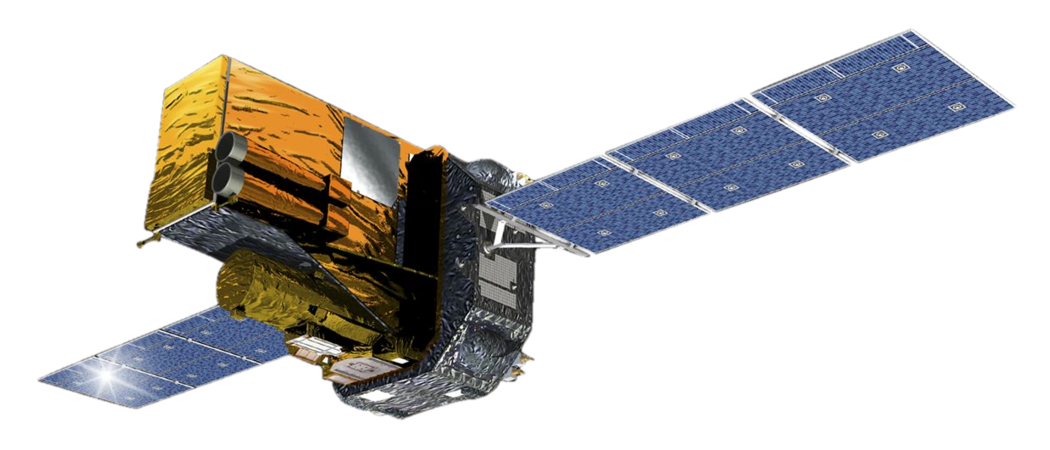
\includegraphics[width = 8cm]{report/Figures/intro/INTEGRAL_spacecraft_model.png}
        \caption{Artist's representation of the \textit{INTEGRAL} telescope.}
        \label{integral}
    \end{figure}
    
        \subsection{JEM-X detector}
        The Joint European Monitor for X-rays (JEM-X) is a complementary detector on-board the \textit{INTEGRAL} telescope. It is primarily used to support the IBIS and SPI instruments in the lower energies for the studies of $\gamma$-ray and X-ray sources. It can however also provide independant scientific results for soft-spectra sources that could be serendipitously detected in the field-of-view(FOV) of the detector. This is the case for Venus here.
        % add a table of jemx parameter and performance. See table 1 of osa_um_jemx.pdf
        The characteristics of JEM-X can be found on \textbf{Tab.} \ref{jemx_perf}. \textbf{Fig.} \ref{jemx}a shows a splitted view of the different constituents of the instrument. \textbf{Fig.} \ref{jemx}b is a top view representation of the coded mask of JEM-X. The instrument actually consists of two of these coded-aperture mask telescope units: JEM-X1 and JEM-X2. Each unit is composed of three parts: the detector, the electronics and the coded mask. For this study, only JEM-X2 data were used.

        The detector of each JEM-X unit consists of a microstrip gas chamber (90\% xenon and 10\% methane at 1.5 bar). The incoming photons are absorbed in the xenon gas by photo-electric absorption and the resulting ionization cloud is then amplified in an avalanche of ionisations by the strong electric field near the microstrip anodes\cite{2020ISDCManual}.

        High-energy electromagnetic radiations cannot be observed using lenses or mirrors. Instead, patterns of materials opaque to the observed wavelengths called \textit{coded-aperture masks} are used. An illustration is shown on \textbf{Fig.} \ref{jemx}b. By blocking the incoming radiation in a pre-determined pattern using mask elements, the image of the source observed casts a shadow on the detector. Reconstruction algorithms are then used to find the position of the source and its intensity\footnote{See \url{https://asd.gsfc.nasa.gov/archive/cai/coded_intr.html\#section2} for details and \cite{Dicke1968SCATTER-HOLERAYS}}. The resolution of the mask is defined by the mask height above the detector and the mask element size. For JEM-X, these a respectively 3.4m and 3.3mm\cite{2020ISDCManual}.

        %explain detector(in osa_um_jemx.pdf) + coded mask(find on internet), don't forget to say that above 5°, the response is too low so the query is only done within 5°.

        \begin{table}[H]
        \centering
        \begin{tabular}{@{}lc@{}}
        \toprule
        \multicolumn{2}{c}{\textbf{JEM-X Performance parameters}} \\ \midrule
        Energy range [keV]                  & 3 - 35              \\
        Detector area/effective [cm$^2$]    & 500/125             \\
        Energy resolution                   & 1.3 keV @ 10 keV    \\
        Field-of-View (FoV)                 & 4.8° (Fully coded)  \\
        Angular resolution (FWHM) [arcmin]  & 3                   \\ 
        Pixel size [arcmin]                 & 1.56               
        \end{tabular}
        \caption{JEM-X key performance parameters. See \href{https://www.cosmos.esa.int/web/integral/instruments-jemx}{here} for more details.}
        \label{jemx_perf}
        \end{table}
        
        \begin{figure}[H]
        \centering
        \begin{subfigure}{.45\textwidth}
            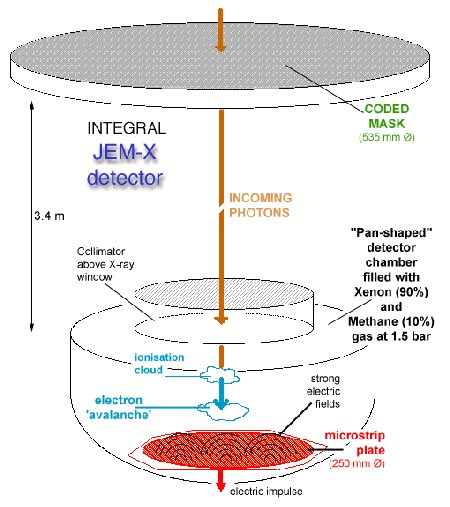
\includegraphics[width=\textwidth]{report/Figures/intro/jem_x_funct_diagram.jpg}
        \end{subfigure}%
        \hspace{1em}-
        \begin{subfigure}{.45\textwidth}
            \centering
            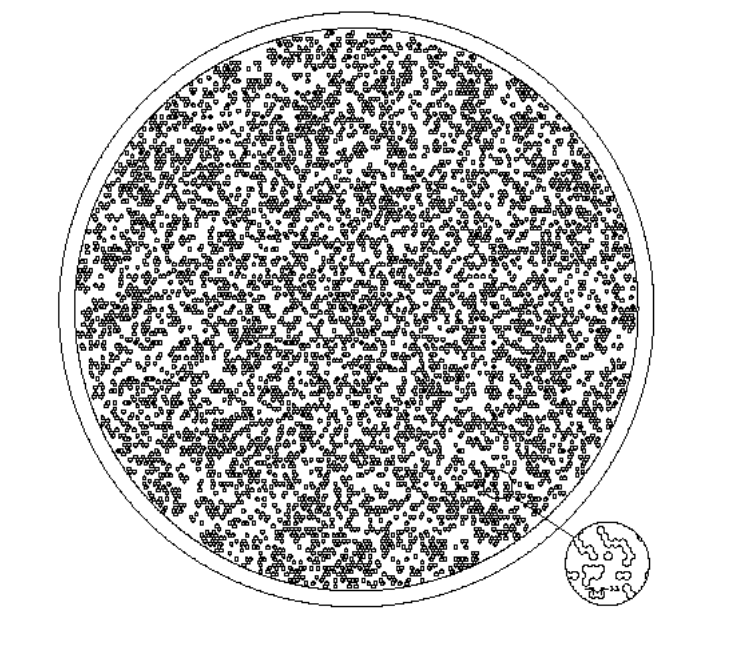
\includegraphics[width=\textwidth]{report/Figures/intro/jemx_coded_mask.png}
        \end{subfigure}
        \caption{(left) Schematic diagram of the different JEM-X constituents. (right) JEM-X's coded mask.}
        \label{jemx}
        \end{figure}
    
    \subsection{\texttt{ODA-API}}

    Spanning more than nineteen years of nearly continuously taken data, the \textit{INTEGRAL} archives contain information on a large number of sources. The mission was initially planned to operate only for five years and the data sets generated were supposed to stay relatively small. But common to scientific space missions, the life of the telescope was extended as long as it stayed functional. The data analysis pipelines for all instruments uses the Offline Science Analysis (OSA) software distributed by the \textit{INTEGRAL} Science Data Centre (ISDC). This software was optimised for the initial mission and the only solution for data processing before \texttt{ODA-API} was via a local installation of OSA on a user computer. Given the amount of data generated since then, the data processing resources now require a significant amount of computing resources. This is why the \texttt{ODA} was developed. It provides an online \textit{INTEGRAL} data analysis system using high-performance and cloud computing technologies accessible through a web browser via the ODA website\footnote{\url{https://www.astro.unige.ch/mmoda/}} or through an API from e.g. a \texttt{Jupyter} notebook by querying the required parameters (see \textbf{List.} \ref{dict} for an example). The \texttt{ODA-API} was used in this study to retrieve the data from the \textit{INTEGRAL} archives.

    \subsection{HEASARC and \textit{INTEGRAL} Science Window Data}

    The High Energy Astrophysics Science Archive Research Center (HEASARC)\footnote{\url{https://heasarc.gsfc.nasa.gov/}} is the primary archive for space missions studying high energy electromagnetic radiations phenomena. The \textit{INTEGRAL} data is queried from the ISDC data servers using the \texttt{astroquery.heasarc} Python interface\footnote{\url{https://astroquery.readthedocs.io/en/latest/heasarc/heasarc.html\#using-alternative-heasarc-servers}}.

    \textit{INTEGRAL}'s activities are splitted into different categories called \textit{windows}. \textit{Science windows} (scw) are what interest us here. Quoting the ISDC, they are continuous time intervals during which all data acquired by the INTEGRAL instruments result from a specific spacecraft attitude orientation state. Scws have different parameters among which their observation identifier (Obs\textunderscore ID) which is a sequence of 11 digits identifying each scw\footnote{See \url{https://heasarc.gsfc.nasa.gov/W3Browse/integral/intscw.html} for more details.}.
    

    \subsection{X-ray emission of planets: the case of Venus}  
    Most planets of our solar system emit in the X-ray domain by interacting with the solar wind(scattering). Most of them are known to shine in the < 3 keV domain. The main emission processes suspected to induce X-ray signal in planetary atmospheres are the following\cite{BhardwajX-raysObjects}:

    \begin{enumerate}
        \item Collisional excitation of neutral species and ions by charged particle impact
        (particularly electrons) followed by line emission.
        \item Brem\ss traslung emission due to electron collisions.
        \item Solar photon scattering: elastic and K-shell fluorescent
        \item Charge exchange of solar wind ions with neutrals
        \item X-ray production from the charge exchange of energetic heavy ions
        with neutrals or by direct collisional excitation of ions.
    \end{enumerate}
    See \cite{BhardwajX-raysObjects} for details about the different processes. Venus is a special planet for that matter as it is deprived of a protecting magnetic field. Studying such a planet is therefore valuable to understand the processes governing the solar wind and atmosphere interaction of planets. Moreover, comets are also deprived of a magnetic field and Venus therefore plays the role of an easily accessible model to understand the impact of the solar wind on these objects
    
    %%talk about processes
    %%talk about why venus is interesting among all.

    Venus has already been observed in the < 3 keV domain notably for the first time with the Chandra telescope\autocite{Dennerl2002DiscoveryChandra}. Venus was expected to be an X-ray emitter due to the verified presence of at least two processes: 3 and 5. In \cite{Dennerl2002DiscoveryChandra}, the planet was clearly detected as a half-lit crescent exhibiting considerable brightening on the sunward limb. The data showed that the emission was dominated by O-K$\alpha$, C-K$\alpha$ fluorescence and N-K$\alpha$ (0.28 keV, 0.53 keV and 0.40 keV). More importantly, the observed fluxes exhibited temporal variability on the scale of minutes. Since the solar flux can vary in a similar fashion, it was expected that these scattered solar X-rays would show the same variability. However the authors didn't find any time correlation between the two fluxes. They explained this result as being due to the fact that solar X-rays are predominantly emitted from localised regions and that Venus was seeing a  46.5°-48° rotated side of the Sun. The solar flux was measured from the GOES satellites orbiting Earth and not Venus. No charge-exchange interactions were measured at these energy ranges and none were expected given the sensitivity of the telescope.

    To observe such charge exchange interactions, Venus was observed during and after it was hit by a powerful interplanetary coronal mass ejection (ICME) in \cite{Xu2019ObservationsEjection}. Heavy ion flux up to 10 keV were observed that were due to charge-exchange interactions with the ICME.

    See \autocite{BhardwajX-raysObjects, Futaana2017SolarAtmosphere} for a great deal of details on the interaction of the solar wind with Venus' atmosphere and solar system planets in general.


%------------------------------------------------

\section{Observation, data analysis and methods}
    \subsection{Data selection}
    \subsection{Models and assumptions}
    \subsection{GOES missions}

%------------------------------------------------
\section{Results}
The results are separated in three sections. First the fluxes from the three different methods are presented. Then, a comparison is made with the Chandra spectra from \cite{Dennerl2002DiscoveryChandra} and with the solar flux variation for the observation window. Finally, the solar event locator is presented.
    \subsection{Fluxes results}

    
    \textbf{22.04.2022}

    \textbf{Fig.} \ref{22_lc} shows the flux obtained with the different methods for the 22.04.2022. The colours of the different data points correspond to the different scws listed in \textbf{Tab.} \ref{journal} in that same order. As one wishes to combine the measurement of the fluxes with differing errors, a weighted average and uncertainty are computed in the following way:

    \begin{align}
        & \mu = \frac{\sum_i\frac{x_i}{\sigma_i^2}}{\sum_i \frac{1}{\sigma_i^2}} \\
        & \sigma(\mu) = \frac{1}{\sum_i\frac{1}{\sigma_i^2}}
    \end{align}

        \begin{figure}[H]
        \centering
        \begin{subfigure}{\textwidth}
            \centering
            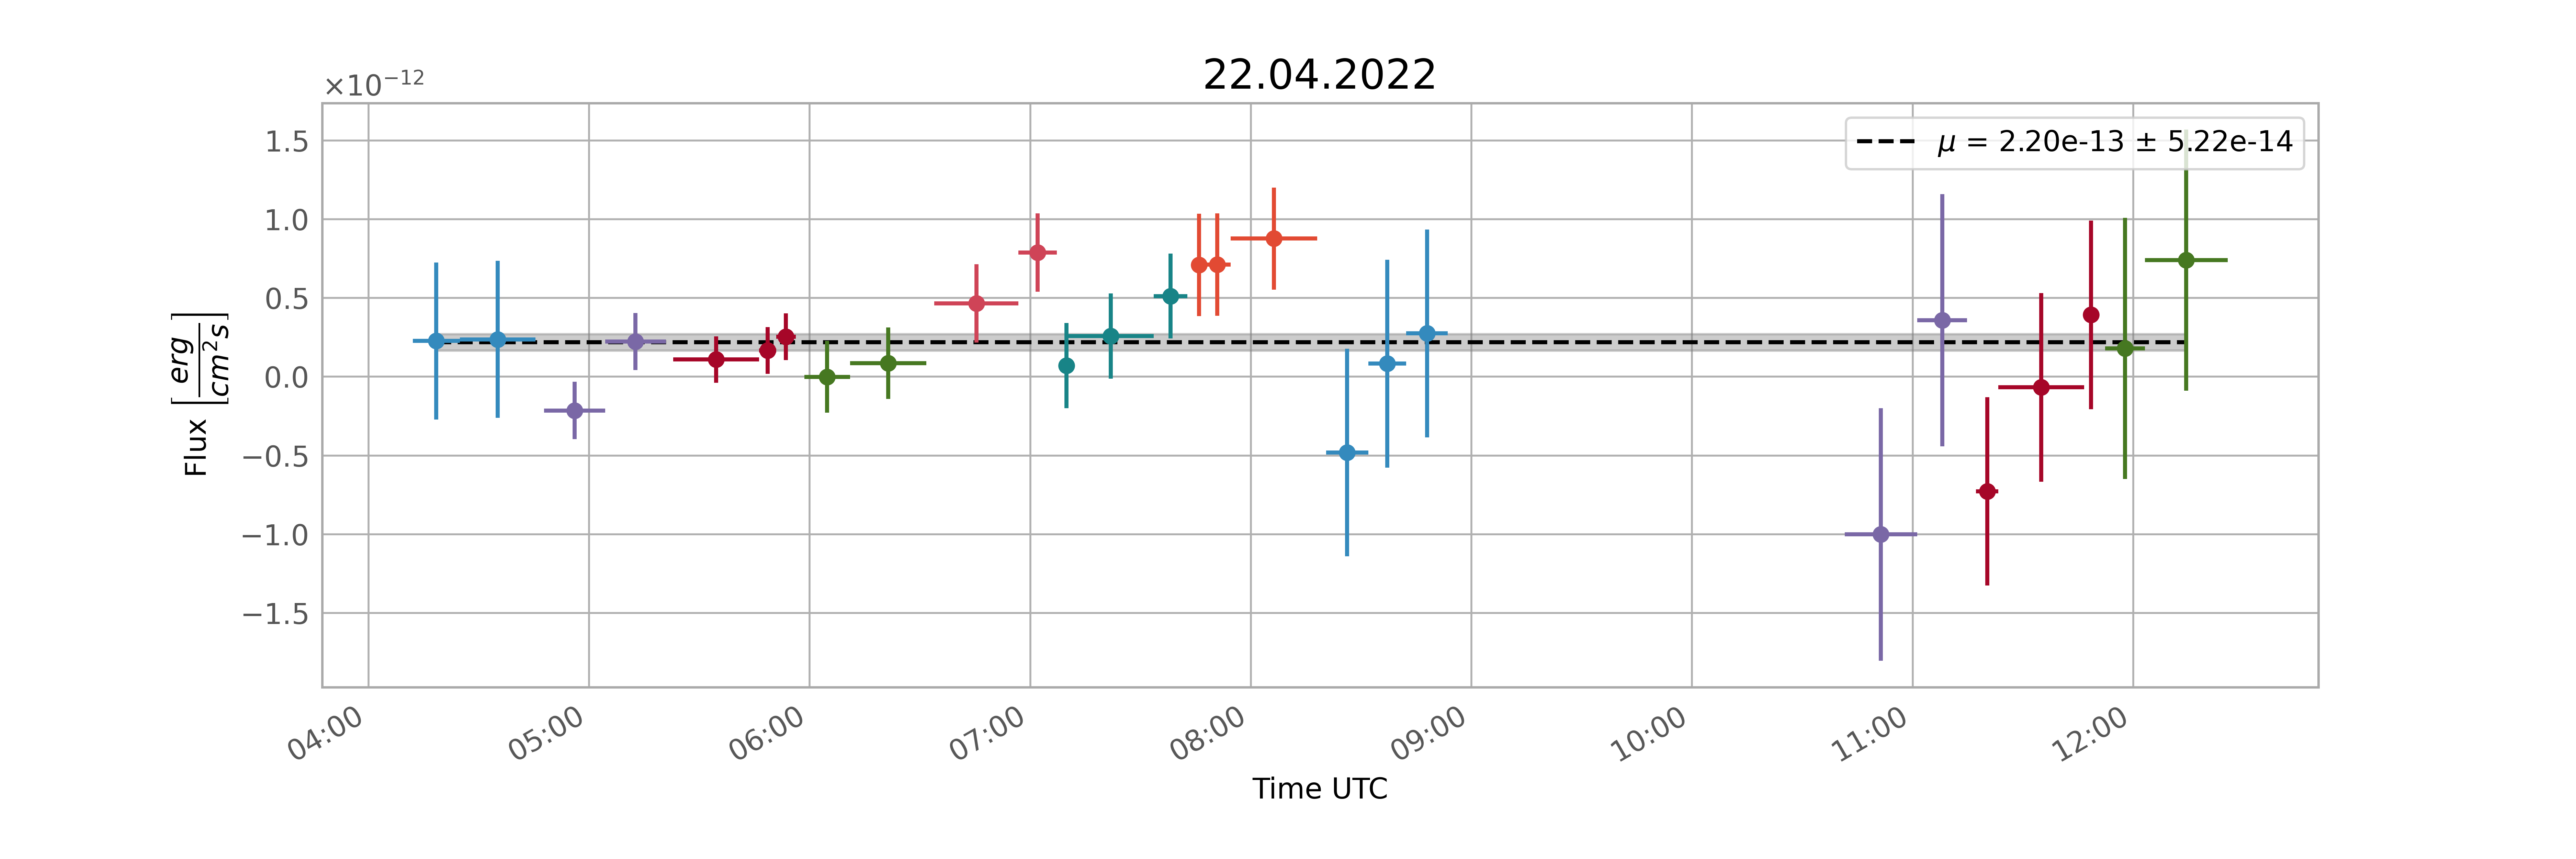
\includegraphics[width=0.8\textwidth]{report/Figures/results/lc_2204.png}
        \end{subfigure}%
        \hspace{1em}
        \begin{subfigure}{\textwidth}
            \centering
            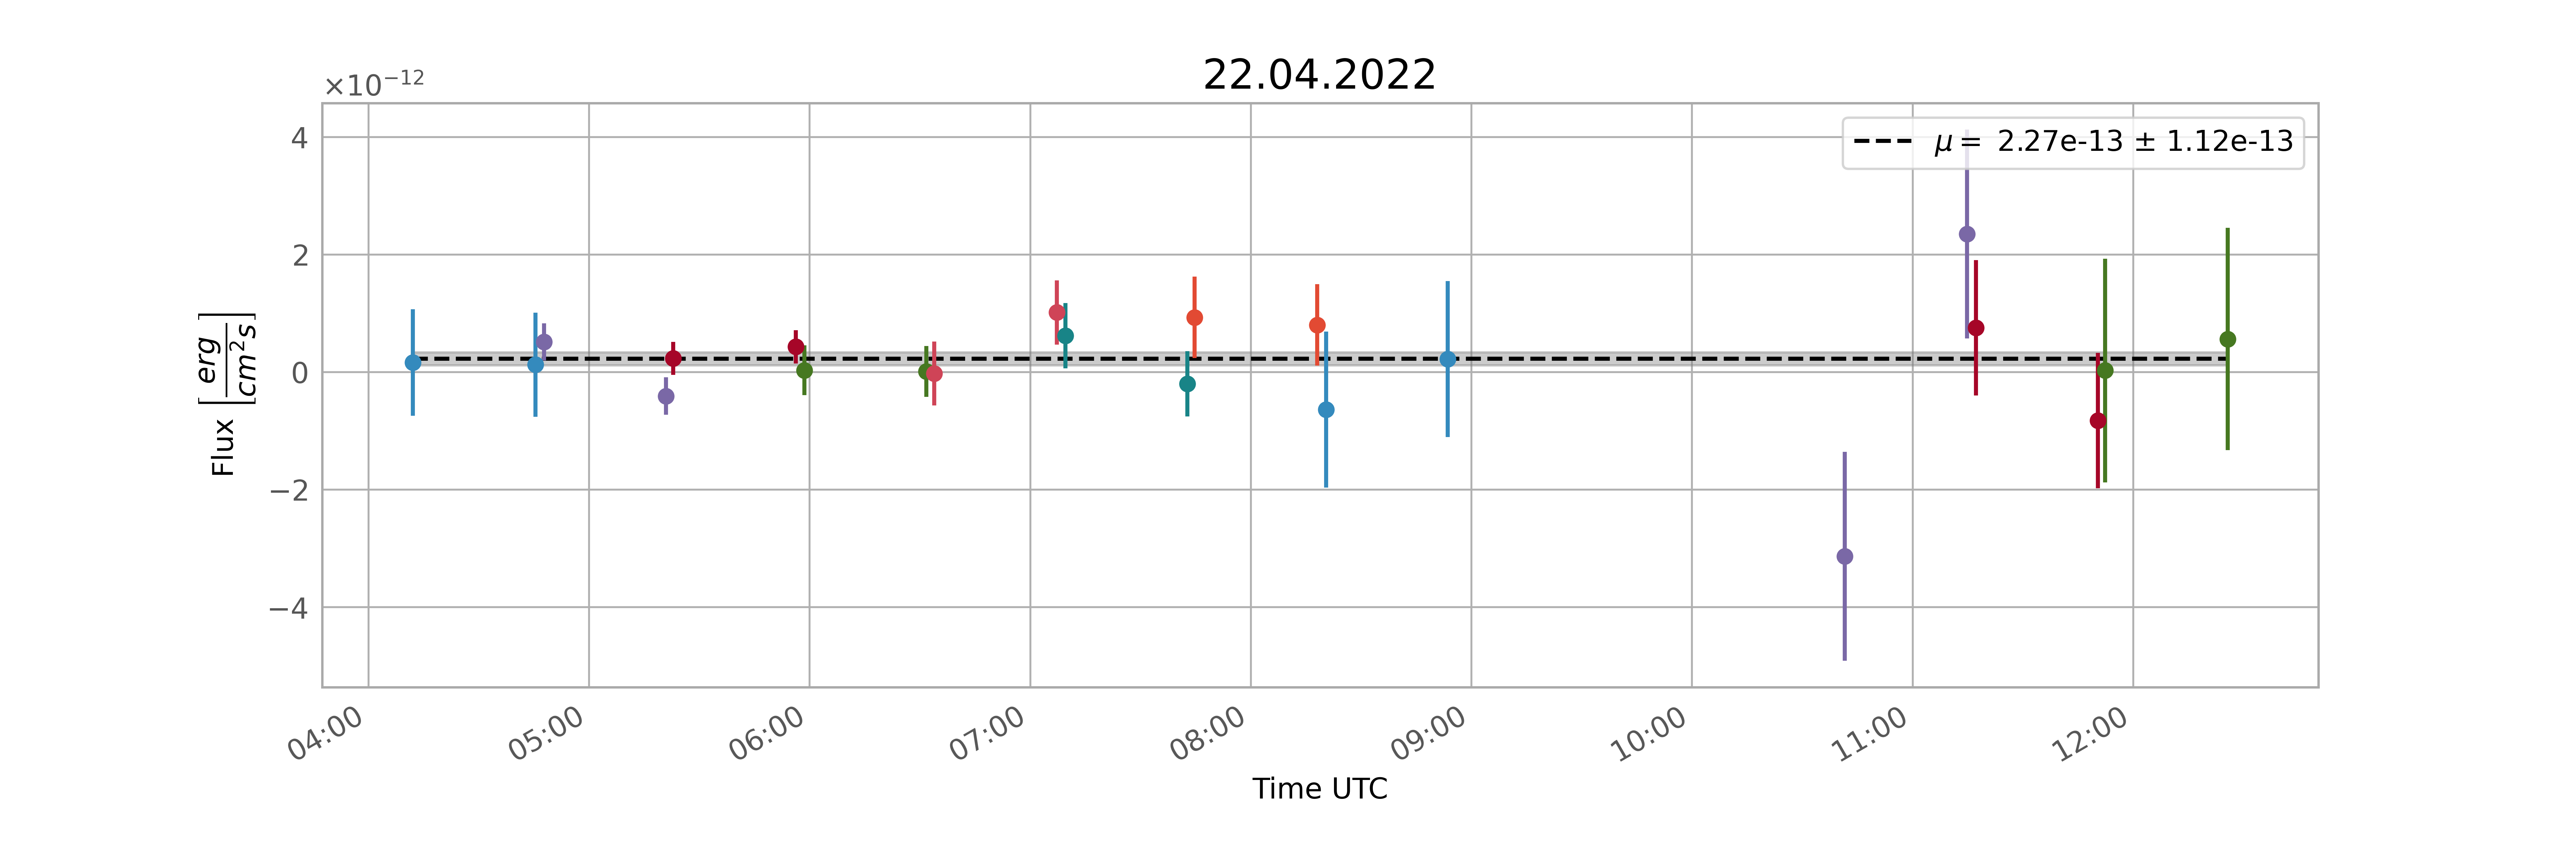
\includegraphics[width=0.8\textwidth]{report/Figures/results/lc_2204_psf_notconst.png}
        \end{subfigure}
        \hspace{1em}
        \begin{subfigure}{\textwidth}
            \centering
            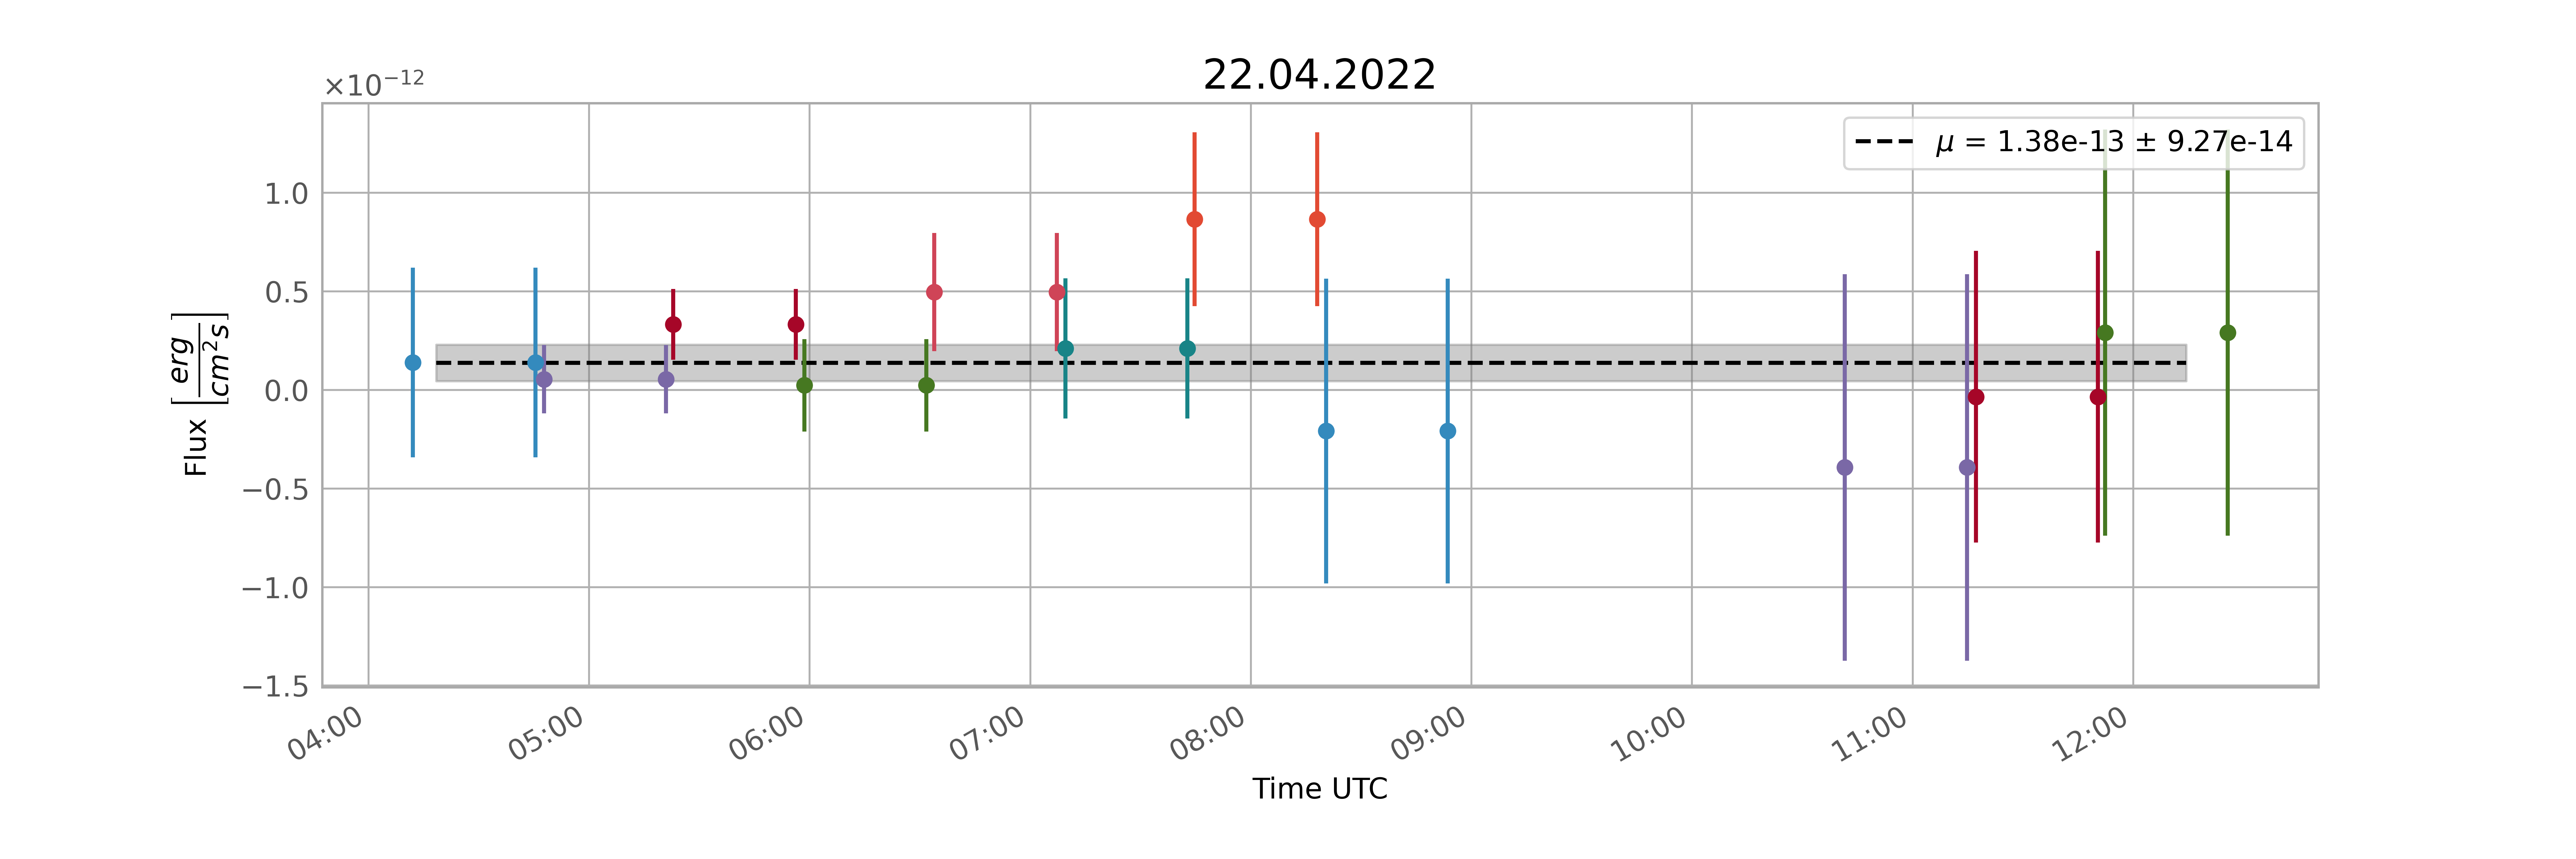
\includegraphics[width=0.8\textwidth]{report/Figures/results/lc_2204_psf_const.png}
        \end{subfigure}
        \caption{For the 22.04.2022, from top to bottom: LC using the pixel value, the non constant PSF model and the constant PSF model.}
        \label{22_lc}
        \end{figure}
        

    \paragraph{24.04.2022}

    The same is done with the 24.04 scws and is shown on \textbf{Fig.} \ref{24_lc}.
    
        \begin{figure}[H]
        \centering
        \begin{subfigure}{\textwidth}
            \centering
            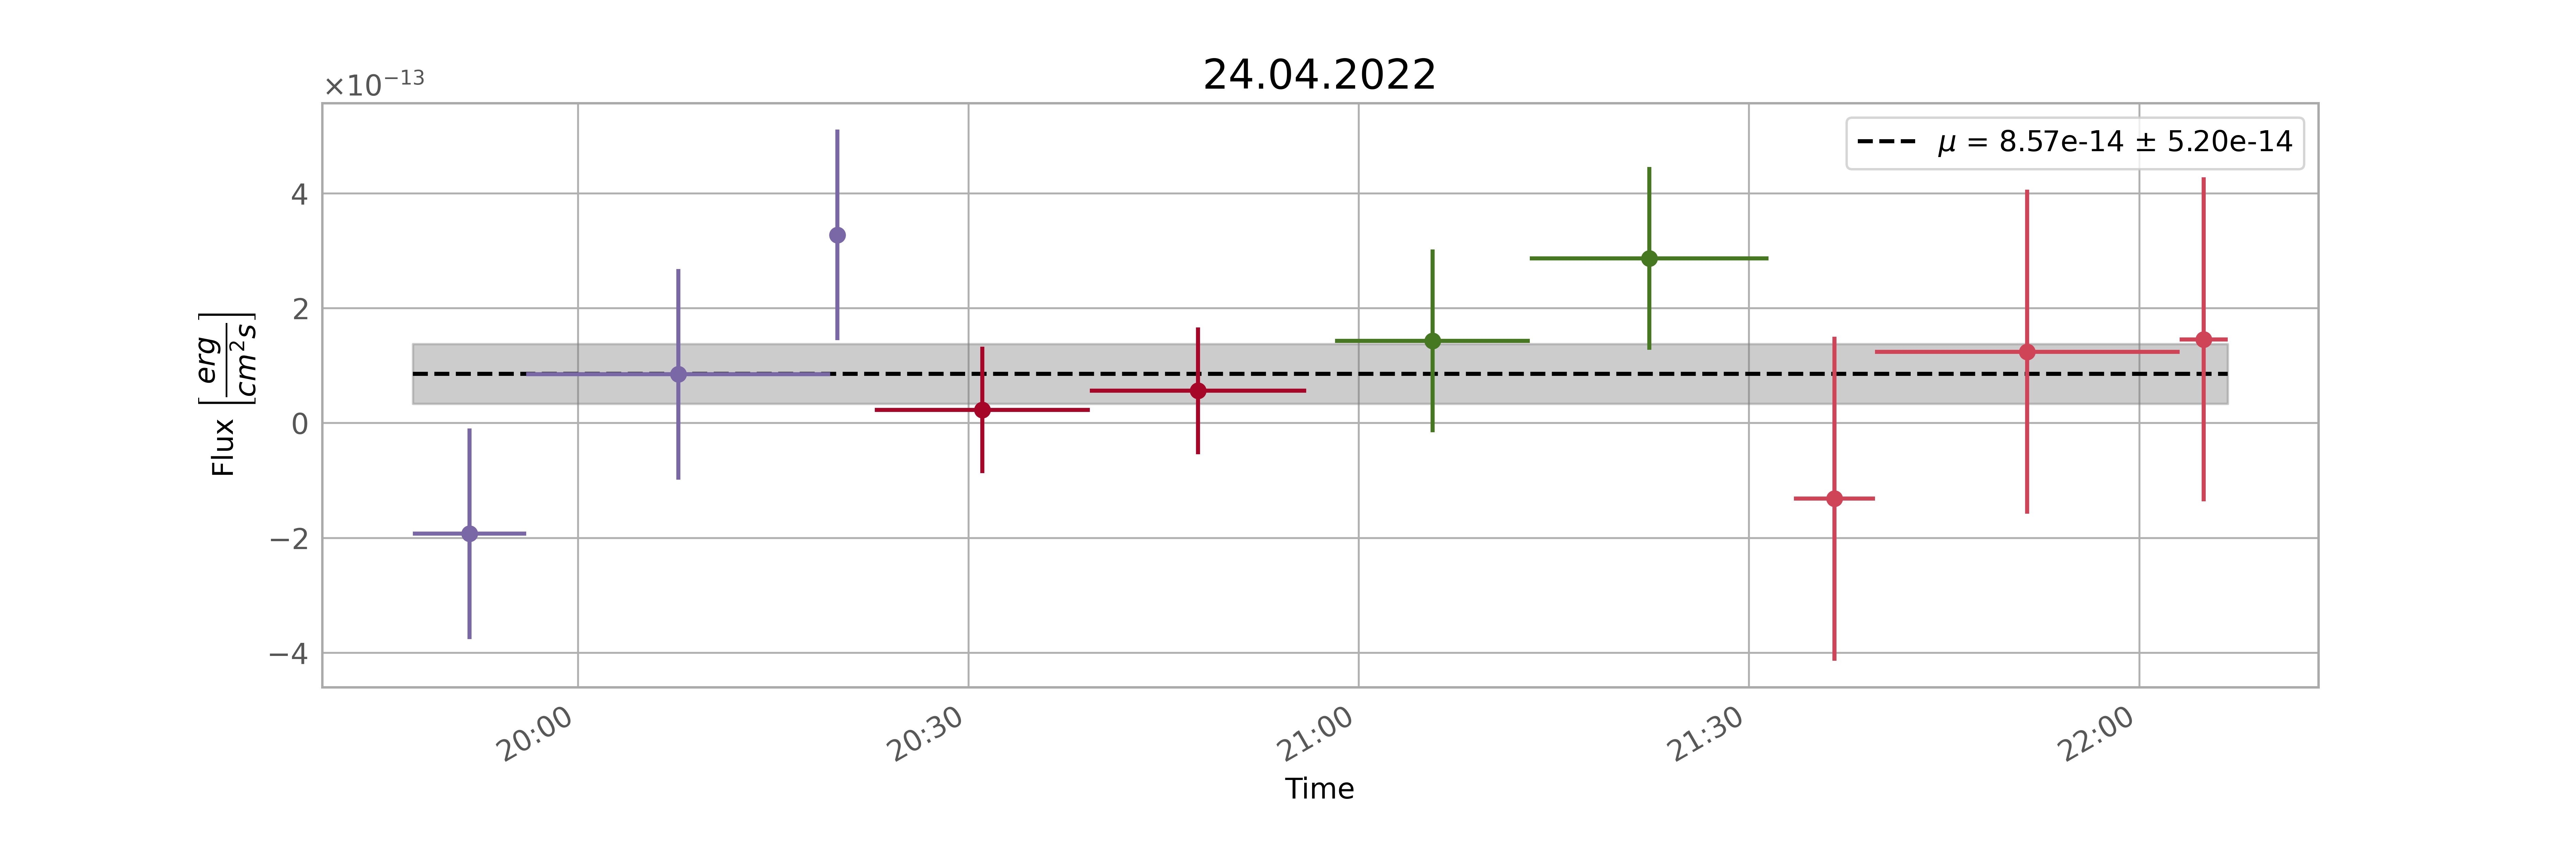
\includegraphics[width=0.8\textwidth]{report/Figures/results/lc_2404.png}
        \end{subfigure}%
        \hspace{1em}
        \begin{subfigure}{\textwidth}
            \centering
            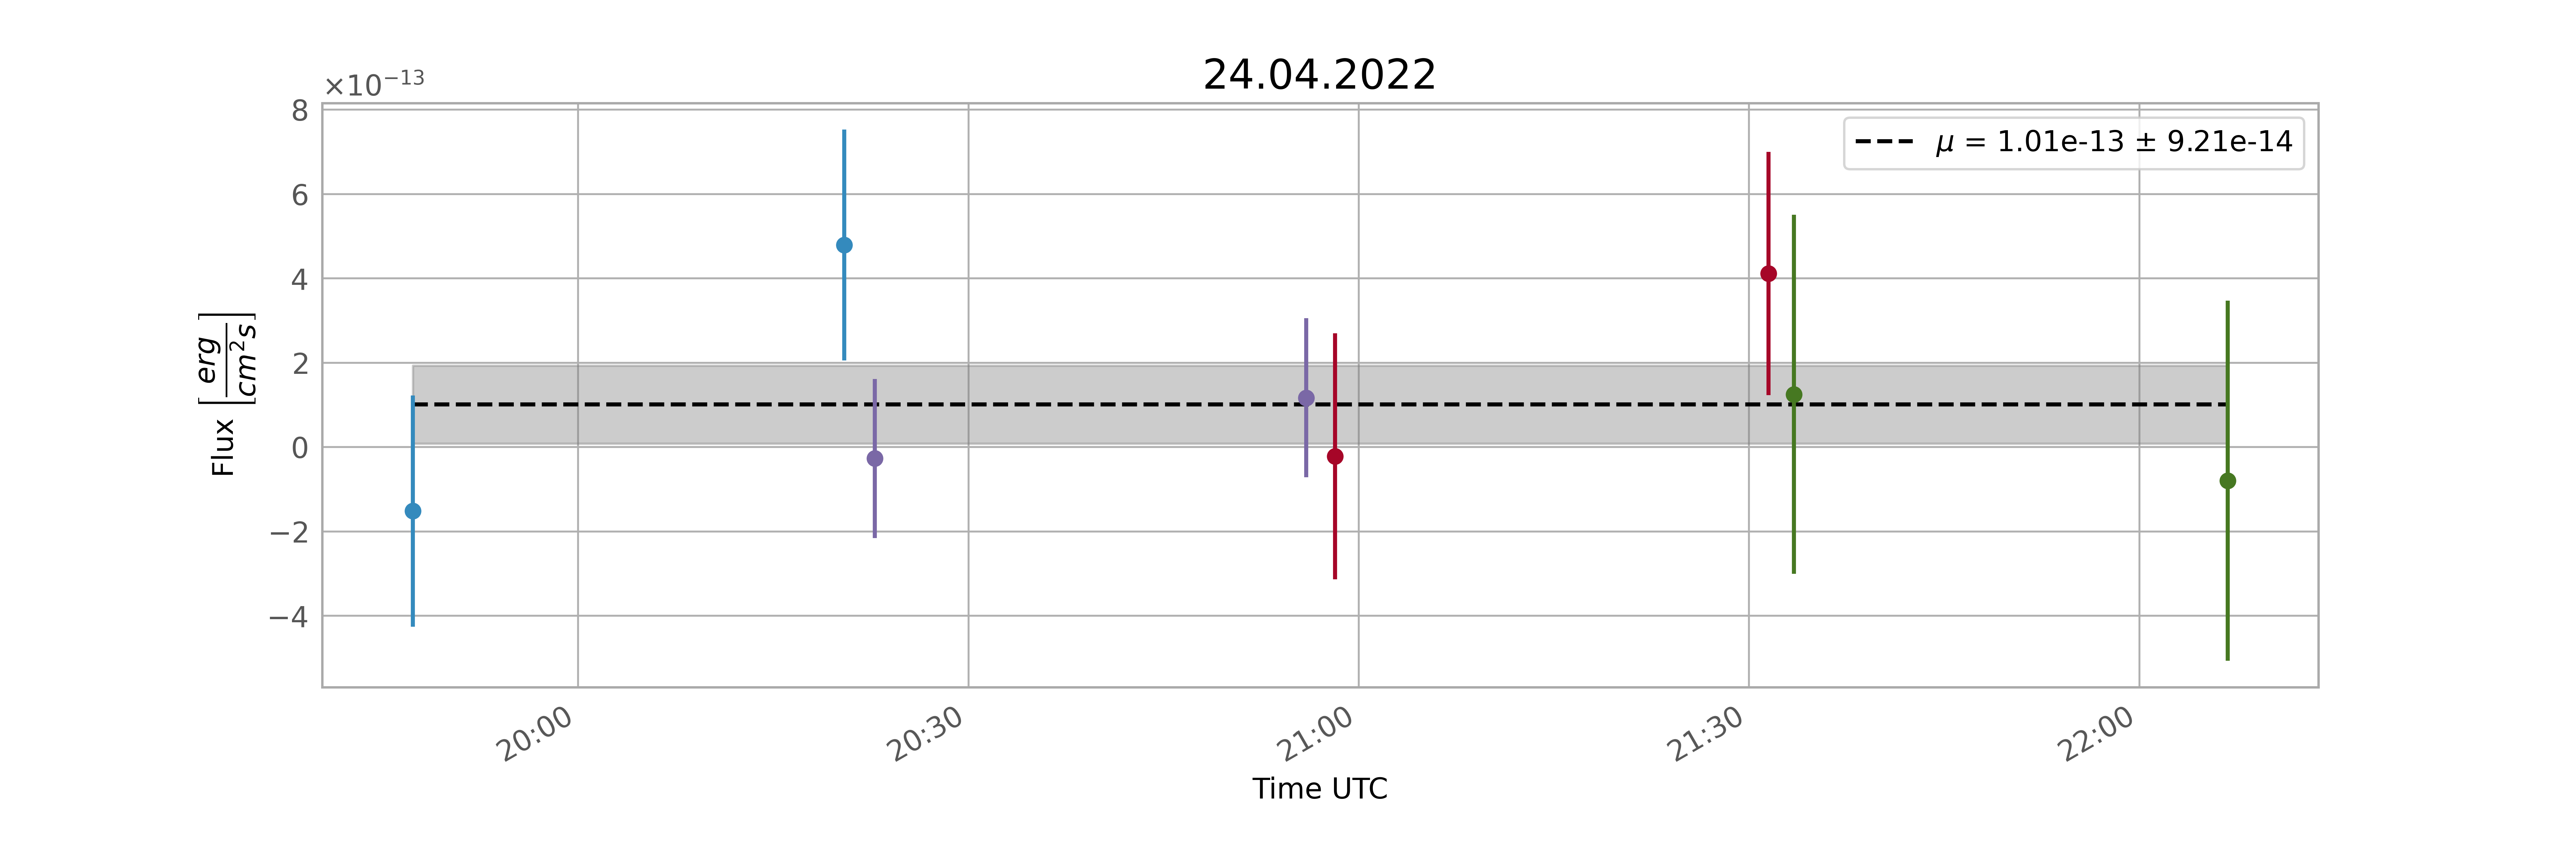
\includegraphics[width=0.8\textwidth]{report/Figures/results/lc_2404_notconst.png}
        \end{subfigure}
        \hspace{1em}
        \begin{subfigure}{\textwidth}
            \centering
            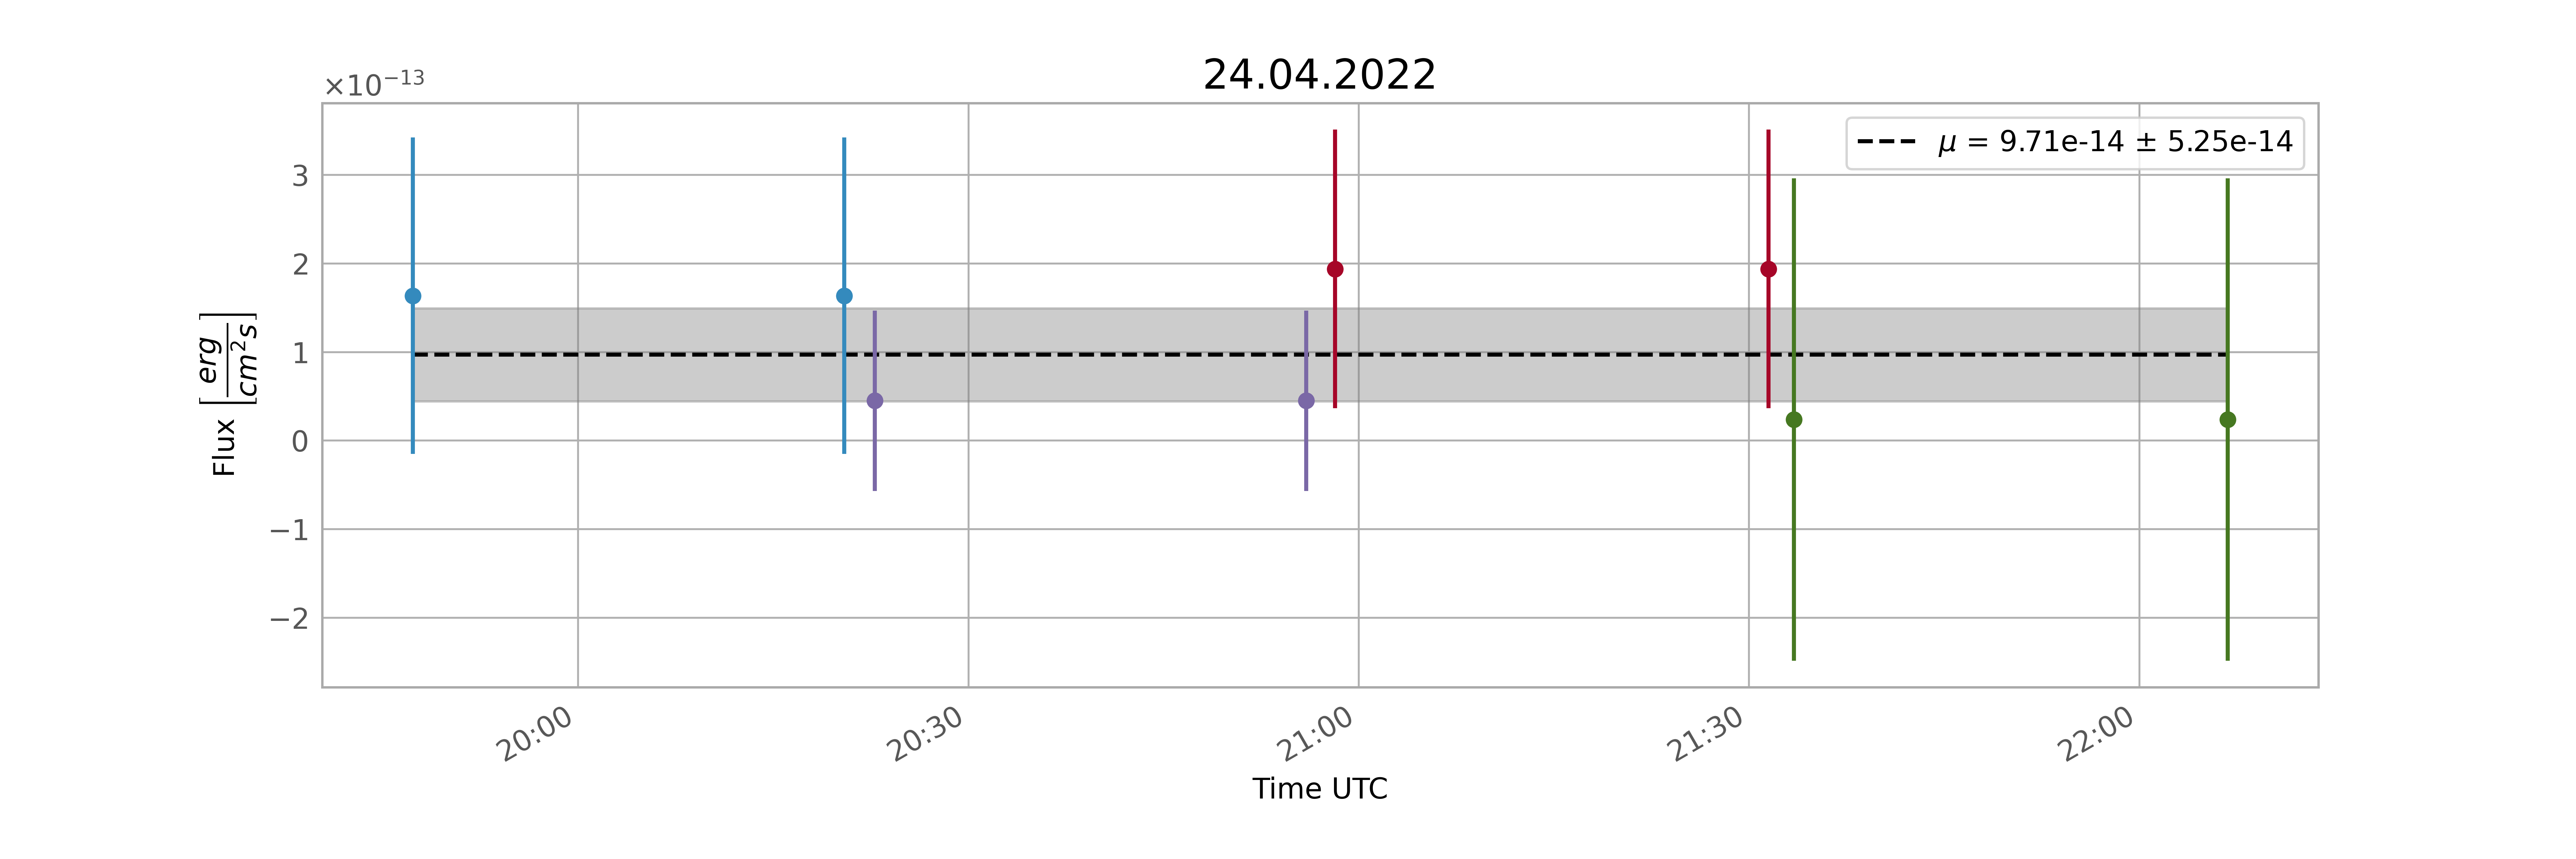
\includegraphics[width=0.8\textwidth]{report/Figures/results/lc_2404_psf_const.png}
        \end{subfigure}
        \caption{For the 24.04.2022, from top to bottom: LC using the pixel value, the non constant PSF model and the constant PSF model.}
        \label{24_lc}
        \end{figure}

    The average fluxes obtained with the first method for both windows are positive at the 3$\sigma$ level as per how JEM-X's variance map is built. For the other two methods, the fluxes are also positive given the 2\% threshold. Moreover, the values obtained between the three different methods are similar and reinforces the idea of a positive average flux observed in both windows.

    \begin{figure}[H]
        \centering
        \begin{subfigure}{0.42\textwidth}
            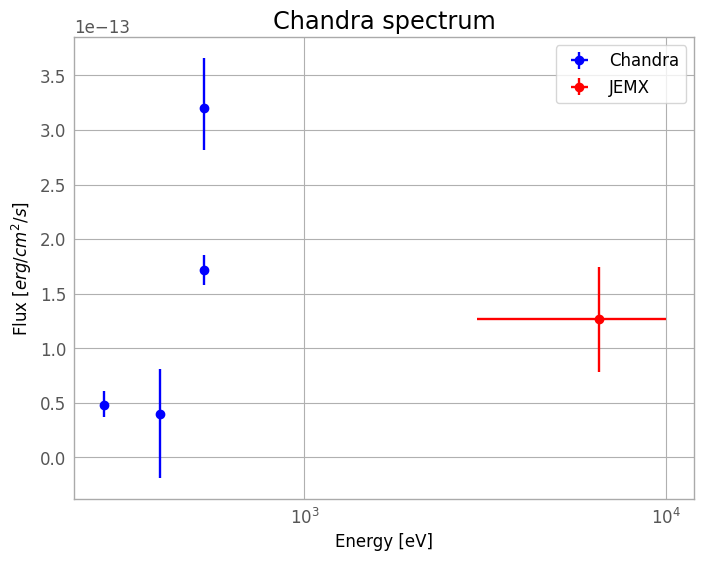
\includegraphics[width=\textwidth]{report/Figures/results/spectra_comp.png}
        \end{subfigure}%
        \hspace{1em}
        \begin{subfigure}{0.42\textwidth}
            \centering
            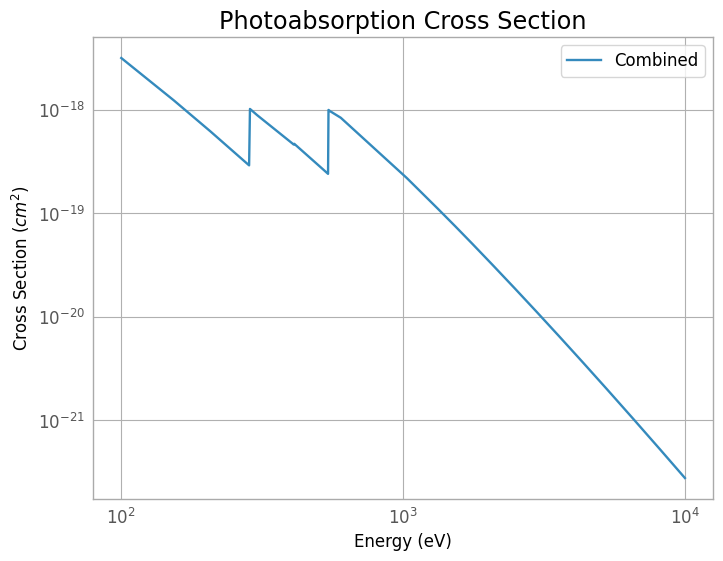
\includegraphics[width=\textwidth]{report/Figures/discussion/crosssection.png}
        \end{subfigure}
        \caption{(left) Comparison between the flux values obtained in \cite{Dennerl2002DiscoveryChandra} and this study. (right) Cross-section model for the Venusian atmosphere using the \texttt{Xraydb.sqlite} database.}
        \label{comp_spec}
    \end{figure}

    A comparison is made between the fluxes obtained in the \cite{Dennerl2002DiscoveryChandra} paper and here. The cross-section for fluorescence would suggest that the flux at higher energies should decrease. However, this is not the case here as shown on \textbf{Fig.} \ref{comp_spec}. This would suggest mainly two things: either the numbers are wrong in a way and do not represent correctly the flux from Venus or there are other physical sources apart from fluorescence that would contribute to Venus' luminosity in these higher energy ranges. For example, charge exchange interactions which could be more present in higher activity periods of the Sun\cite{BhardwajX-raysObjects}.
    
    \subsection{Concordance with solar flux variations}

    Given that the Sun's flux variability is of the order of minutes and that it is the main X-ray emitting cause on Venus, it is interesting to compare its time variability with Venus' which also varies on a timescale of minutes\cite{Dennerl2002DiscoveryChandra}. The GOES-16 solar flux at 1 A.U. in the XRSA channel is shown at the top of \textbf{Fig.} \ref{goes22} and \ref{goes_24}. The time of each scw is plotted using the same colour code as before on these graphs.
    \begin{figure}[H]
        \centering
        \begin{subfigure}{0.9\textwidth}
        \centering
            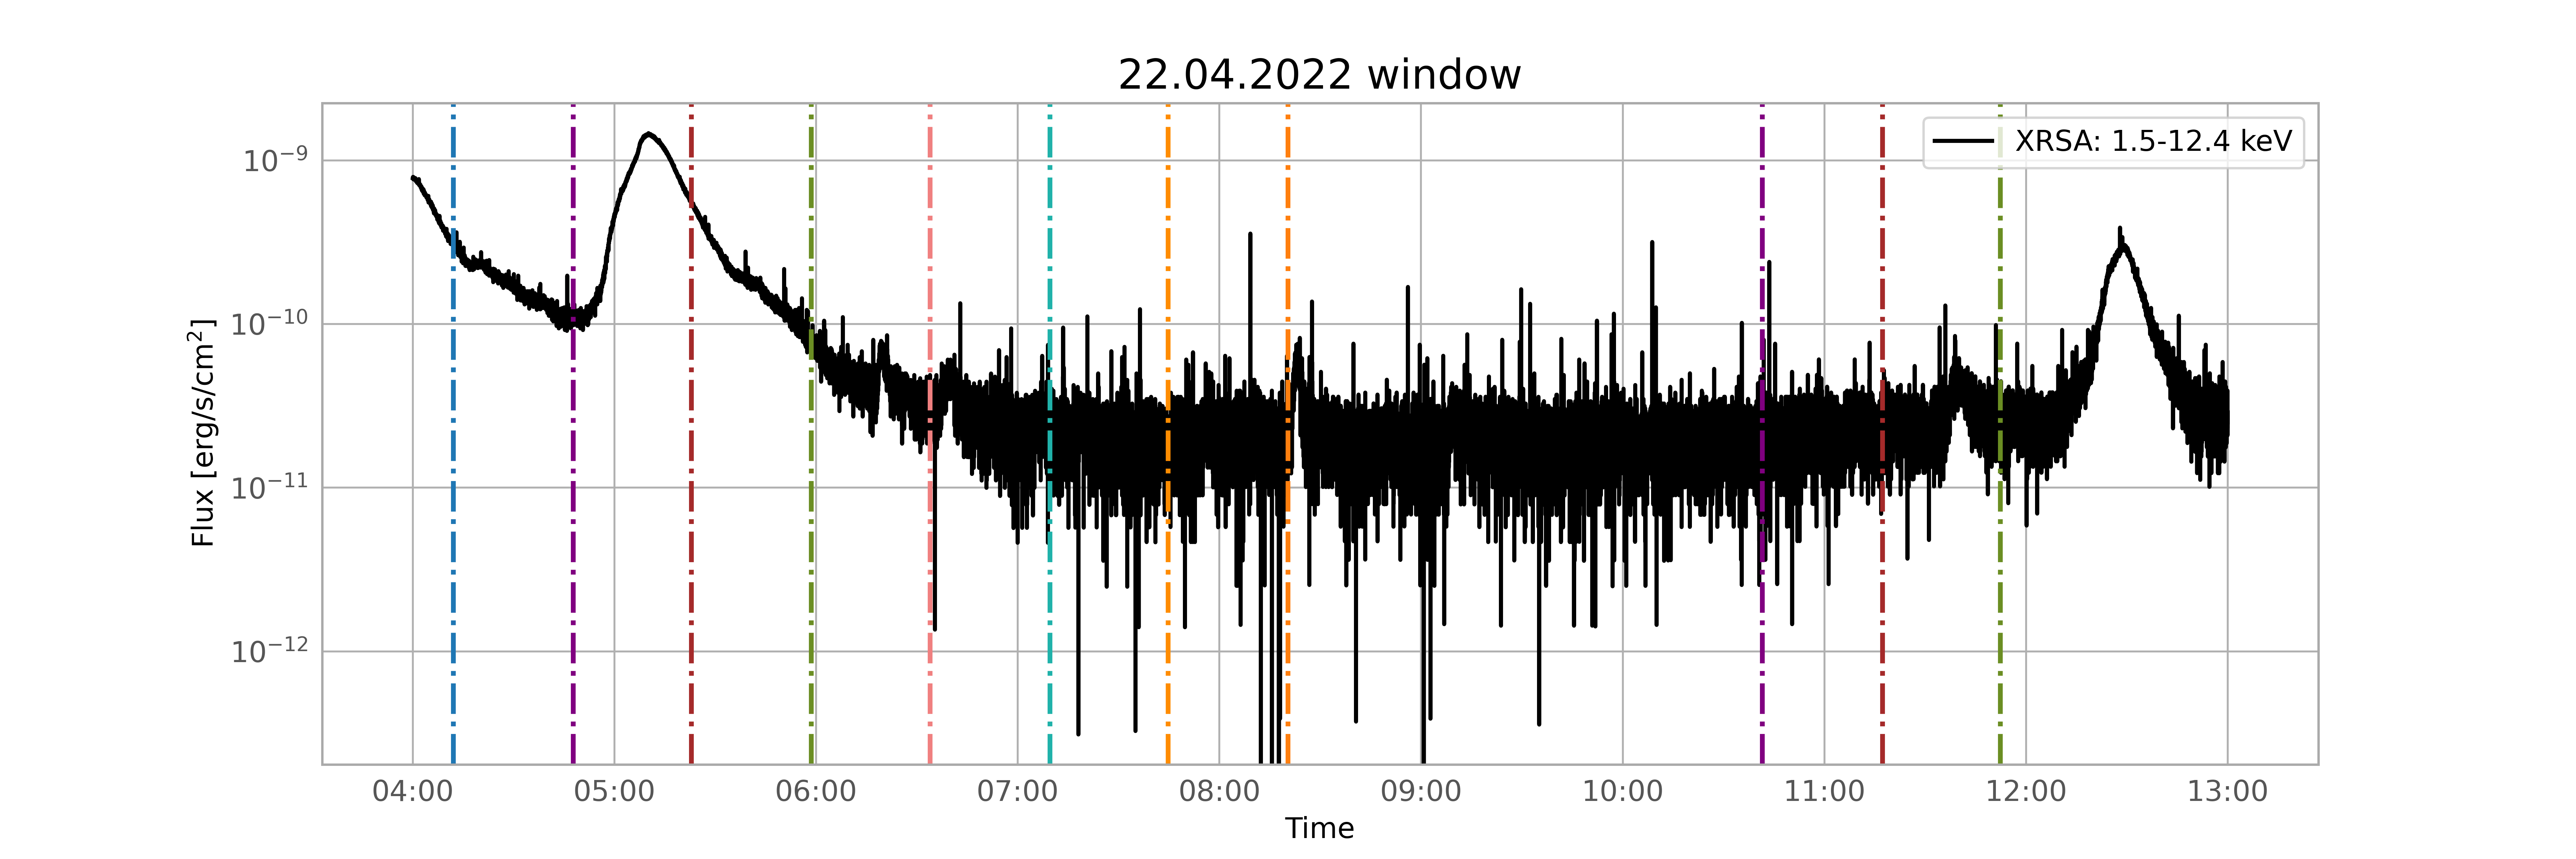
\includegraphics[width=\textwidth]{report/Figures/results/GOES_22.png}
        \end{subfigure}%
        \hspace{1em}
        \begin{subfigure}{0.75\textwidth}
            \centering
            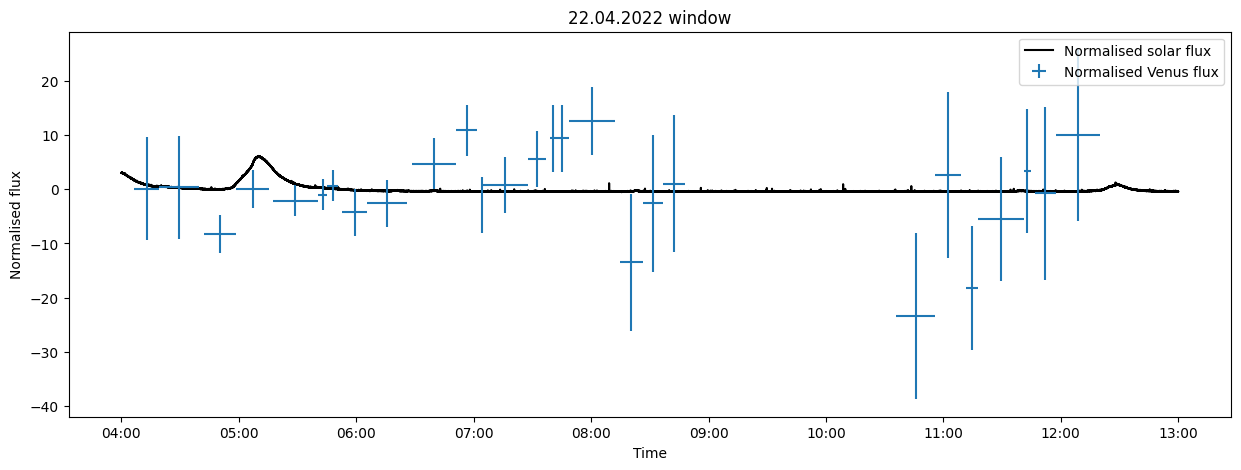
\includegraphics[width=\textwidth]{report/Figures/results/norm_22.png}
        \end{subfigure}
        \caption{Top: 22.04.2022 scws restricted view of the solar flux in the XRSA channel of GOES-16 overplotted with the times of the LC points.
        Bottom: Normalised solar and Venus fluxes plotted together. The data point times were corrected from light travel.}
        \label{goes22}
    \end{figure}


\begin{figure}[H]
    \centering
    \begin{subfigure}{0.9\textwidth}
        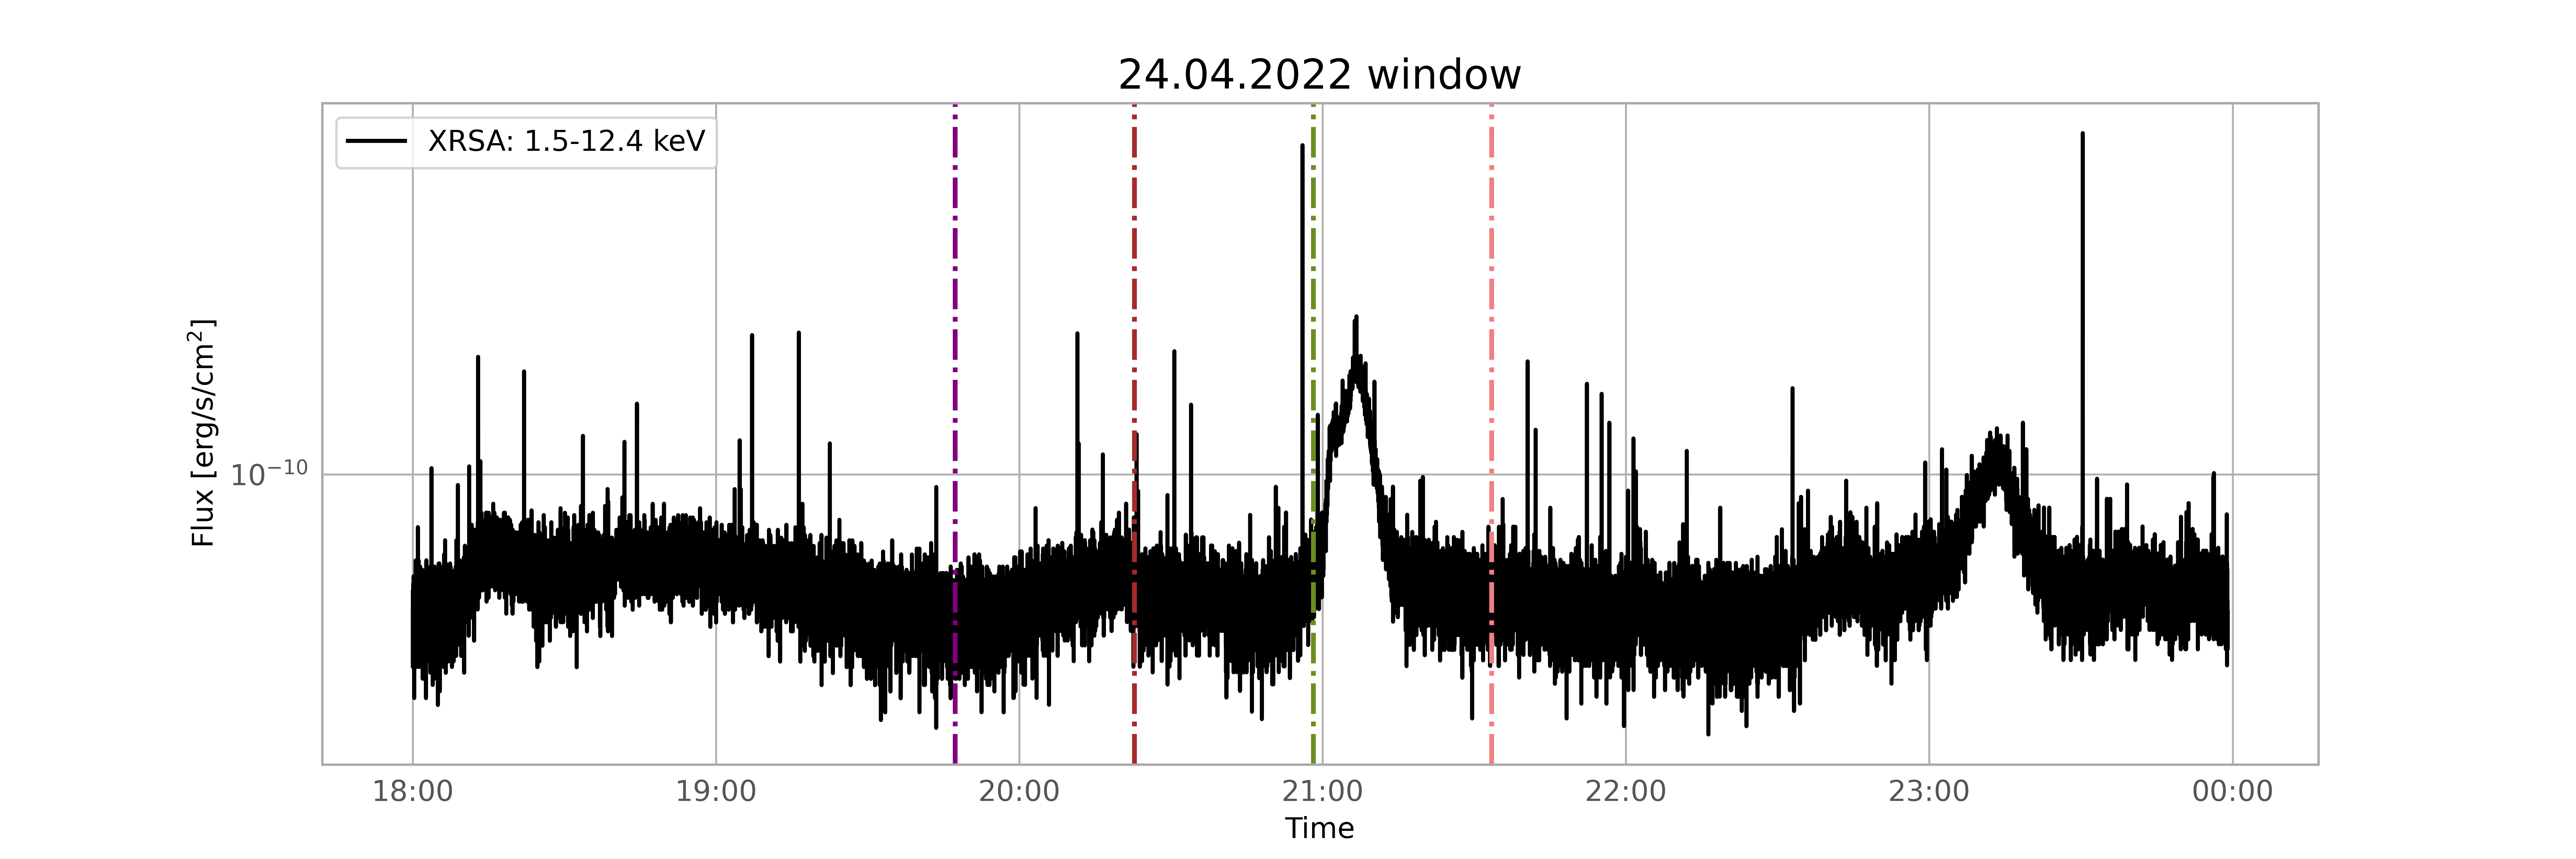
\includegraphics[width=\textwidth]{report/Figures/results/GOES_24.png}
    \end{subfigure}%
    \caption{Top: 24.04.2022 scws restricted view of the solar flux in the XRSA channel of GOES-16 overplotted with the times of the LC points.}
    \label{goes_24}
\end{figure}

\begin{figure}[H]
    \ContinuedFloat
    \centering
    \begin{subfigure}{0.75\textwidth}
        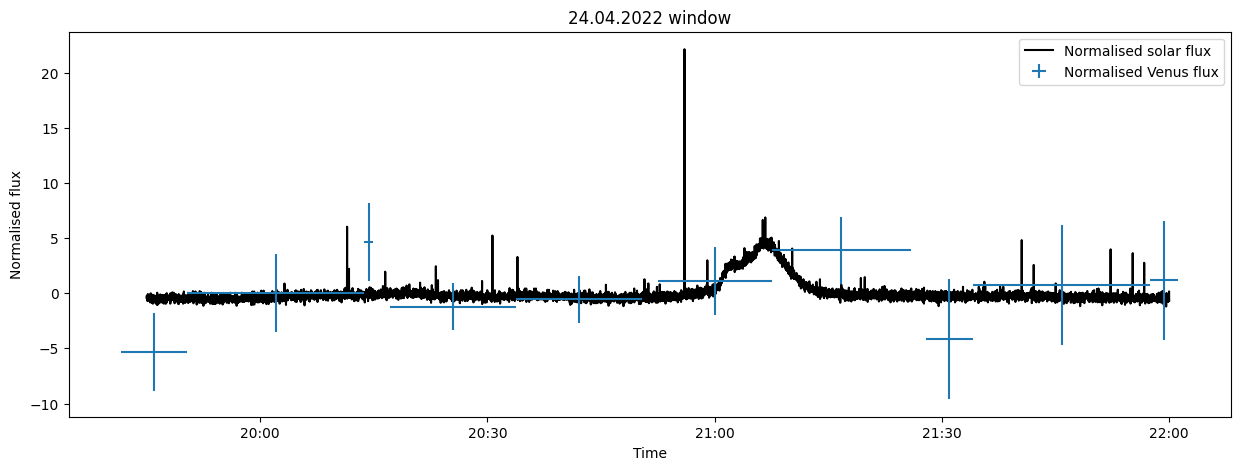
\includegraphics[width=\textwidth]{report/Figures/results/norm_24.png}
    \end{subfigure}
    \caption*{(continued) Bottom: Normalised solar and Venus fluxes plotted together. The data point times were corrected from light travel.}
\end{figure}

Moreover, Venus flux and the solar flux are normalised and plotted together on the bottom side of \textbf{Fig.} \ref{goes22} and \ref{goes_24}. The idea here is to inspect the time correlation between both quantities.  The data points were corrected from light travel time. For the solar flux, the path is: Sun $\rightarrow$ Earth. For the Venus flux, it is: Sun $\rightarrow$ Venus $\rightarrow$ Earth. The data points are 5.6 minutes late on the solar flux data. A two-sample Kolmogorov-Smirnov test is performed on these sample. The significance level is set at a standard 5\%. The results are p-values of 2.6\% and 4.8\% for respectively the 22.04.2022 and the 24.04.2022 windows.

The estimated average energy deposited on Venus in X-ray from the first scw to the last for each day and for the three different methods is given by: 

\begin{equation}
    E = \frac{\pi r_{\venus}^2\mu \Delta t}{illumination},
\end{equation}
where $r_{\venus}$ is Venus' radius and $\Delta t$ is the duration from the first scw to the last on one of the two days observed. The results are the following:

\begin{table}[H]
\centering
\begin{tabular}{@{}lcc@{}}
\toprule
\textbf{Method/Date}             & 22.04.2022    & 24.04.2022     \\ \midrule
Duration [s]                     & 29618         & 8370           \\
Pixel value [$10^{16}$ erg]      & 1.15 $\pm$ 0.27 & 0.13 $\pm$ 0.077 \\
Constant PSF [$10^{16}$ erg] & 0.72 $\pm$ 0.14 & 0.14 $\pm$ 0.077 \\
Non-constant PSF [$10^{16}$ erg]     & 1.18 $\pm$ 0.58 & 0.15 $\pm$ 0.13  \\ \bottomrule
\end{tabular}
\caption{Estimated energy deposited on Venus given the three flux methods.}
\label{depo}
\end{table}

The results all overlapped except for the 22.04.2022 window with the constant PSF method.

    % talk about estimated energy deposited on venus too.
    
    \subsection{Solar events locations}
    The direction of propagation of the solar flares and CMEs are estimated in the HGS thanks to the HEK data based on the HPC coordinates given by the GOES satellite for the flares and the LASCO instrument on SOHO for the CMEs. The model is as simplistic as it can get but it is a first try at such as estimation. A line is drawn between the centre of the Sun and the surface coordinates of the event. The results are shown on \textbf{Fig.} \ref{locator}. The events' directions are clearly biased and this is discussed in the next section. 
    
    \textbf{Fig.} \ref{Mclass_flare} shows an image of the M1.1 class flare detected as the first peak on the 22.04.2022 solar flux plot on \textbf{Fig.} \ref{goes22} by the AIA imager.

        \begin{figure}[H]
        \centering
        \begin{subfigure}{.47\textwidth}
            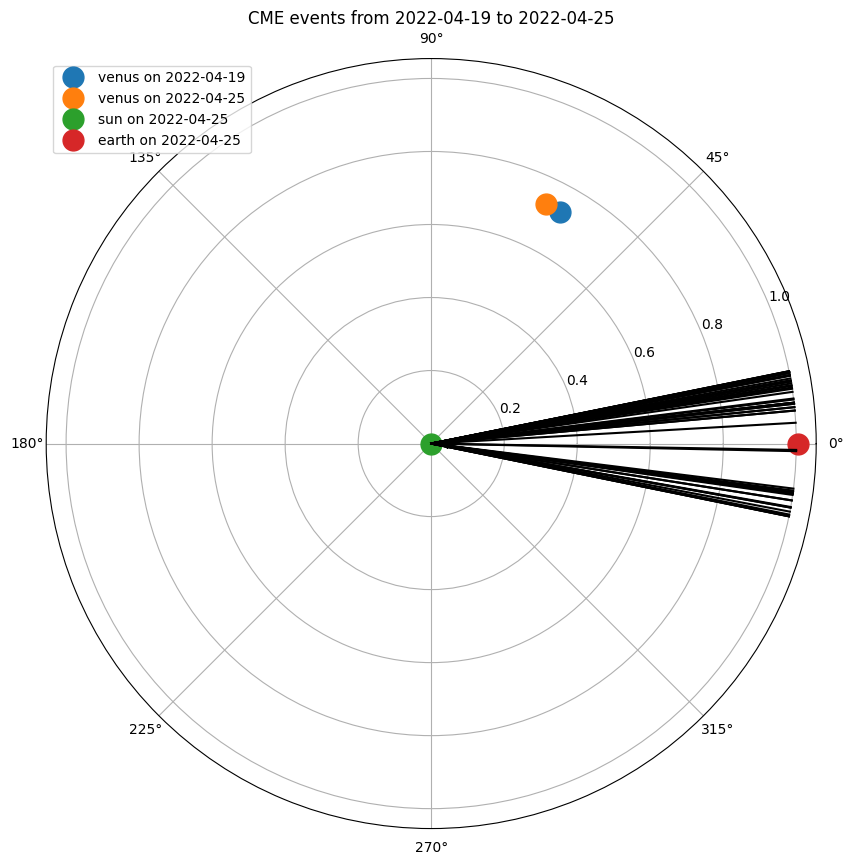
\includegraphics[width=\textwidth]{report/Figures/results/cme_loc.png}
        \end{subfigure}%
        \hspace{1em}
        \begin{subfigure}{.47\textwidth}
            \centering
            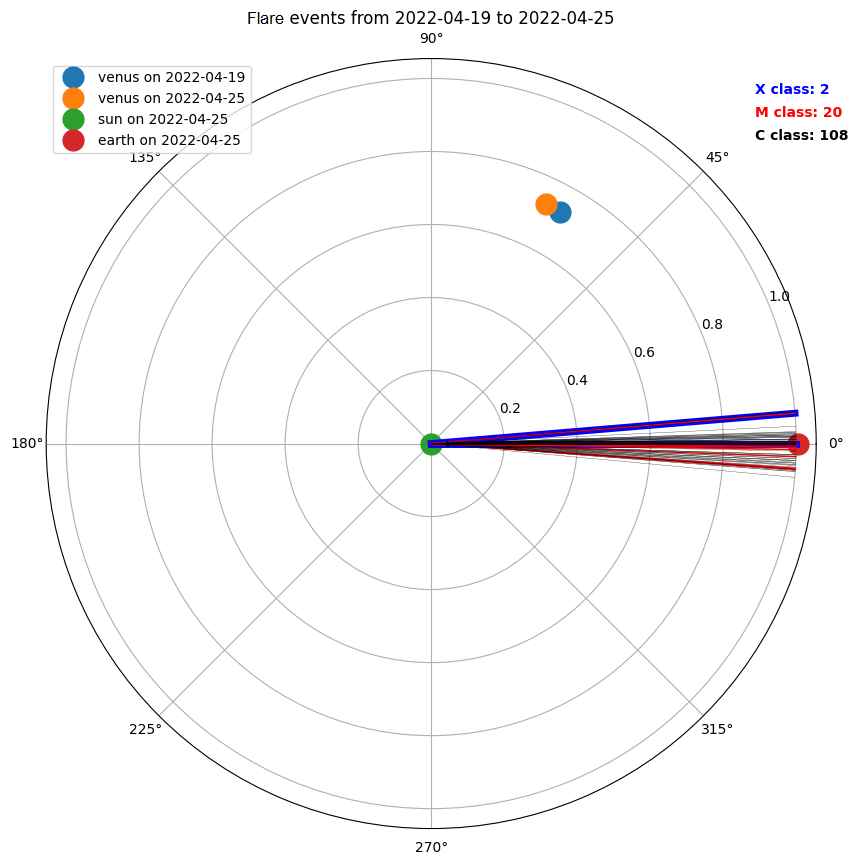
\includegraphics[width=\textwidth]{report/Figures/results/fl_loc.png}
        \end{subfigure}
        \caption{For the 19.04.2022 to 25.04.2022 period: (left) Propagation directions of all CMEs contained in the HEK. (right) Propagation directions of all flares contained in the HEK. The classes of the flares and numbers are indicated in colors.}
        \label{locator}
        \end{figure}

    \begin{figure}[H]
        \centering
        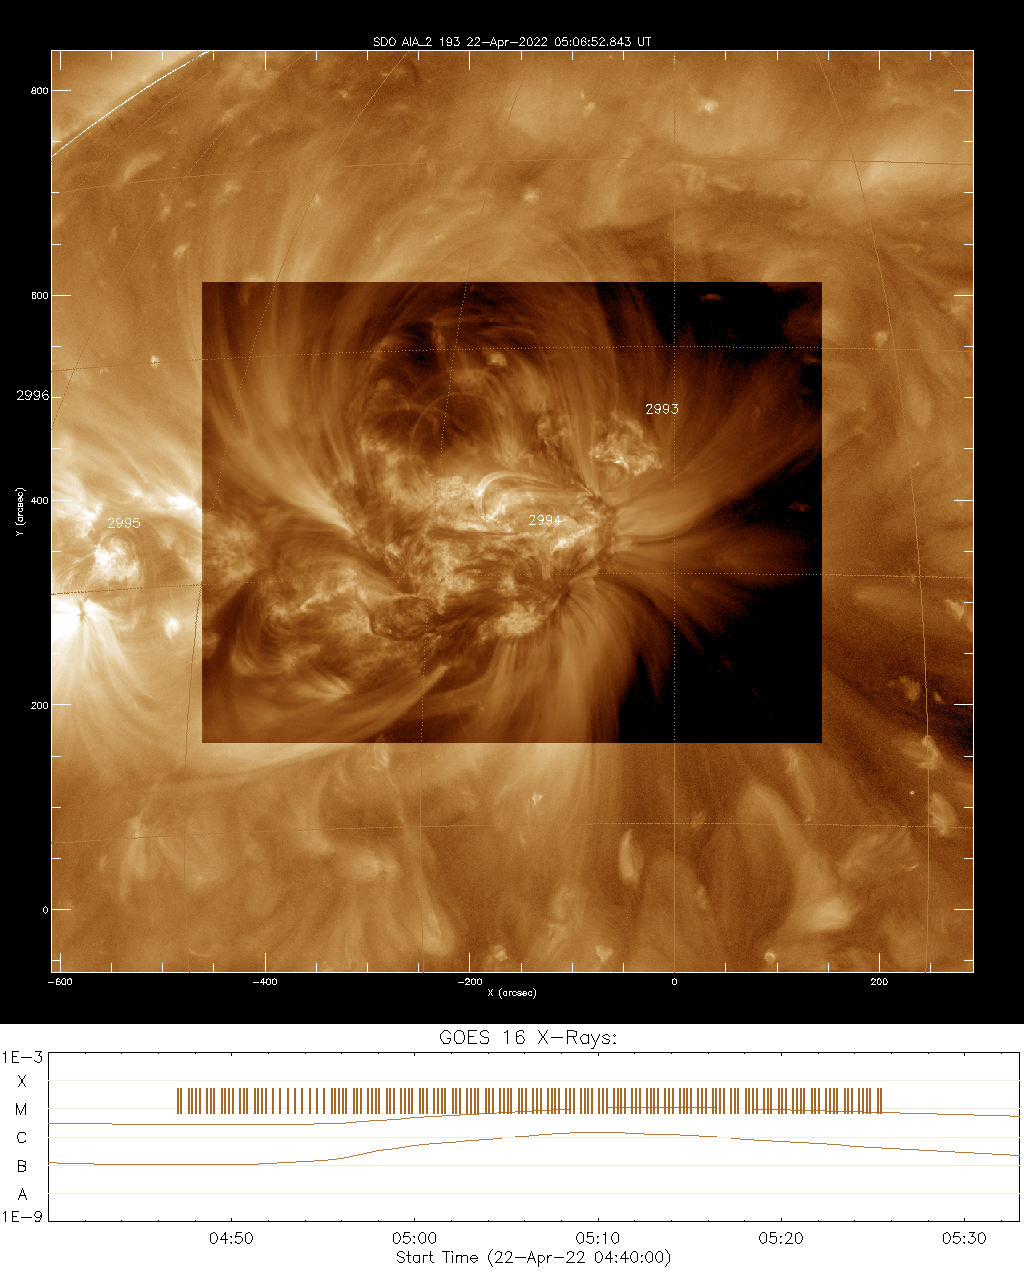
\includegraphics[width = 10cm]{report/Figures/results/aia_Mclass_2204.png}
        \caption{AIA image of the M1.1 class flare visible in the 22.04.2022 window.}
        \label{Mclass_flare}
    \end{figure}

%------------------------------------------------

\section{Discussion}

\begin{table*} % Full width table (notice the starred environment)
	\caption{Example two column table with fixed-width columns.}
	\centering % Horizontally center the table
	\begin{tabular}{L{0.2\linewidth} L{0.2\linewidth} R{0.15\linewidth}} % Manually specify column alignments with L{}, R{} or C{} and widths as a fixed amount, usually as a proportion of \linewidth
		\toprule
		\multicolumn{2}{c}{Location} \\
		\cmidrule(r){1-2}
		East Distance & West Distance & Count \\
		\midrule
		100km & 200km & 422 \\
		350km & 1000km & 1833 \\
		600km & 1200km & 890 \\
		\bottomrule
	\end{tabular}
\end{table*}

\begin{figure} % Single column figure
	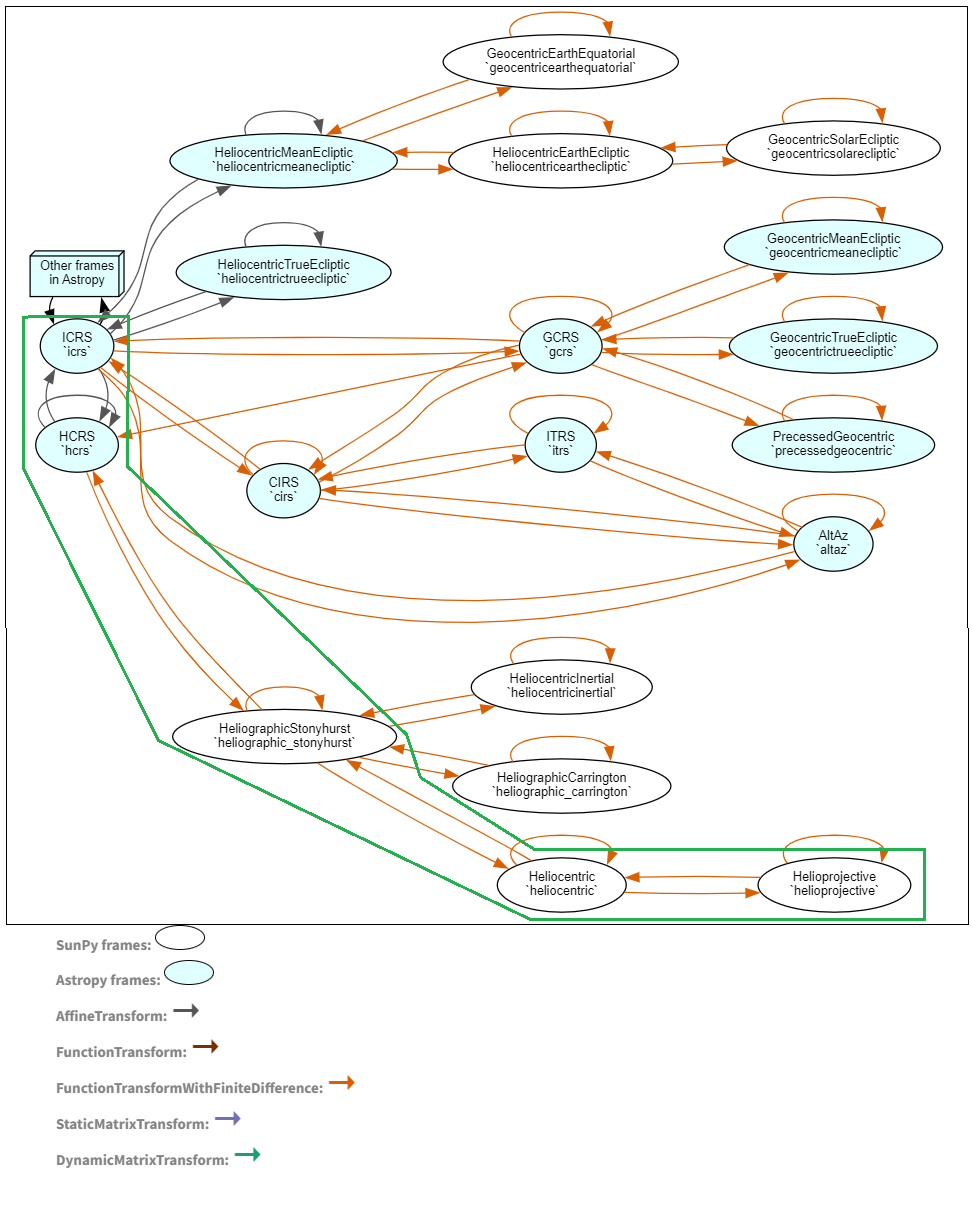
\includegraphics[width=\linewidth]{report/Figures/methods/coordinates.png}
	\caption{Anther of thale cress (Arabidopsis thaliana), fluorescence micrograph. Source: Heiti Paves, \href{https://commons.wikimedia.org/wiki/File:Tolmukapea.jpg}{https://commons.wiki-\\media.org/wiki/File:Tolmukapea.jpg}.}
	\label{fig:tcanther}
\end{figure}

\begin{figure*} % Two column figure (notice the starred environment)
	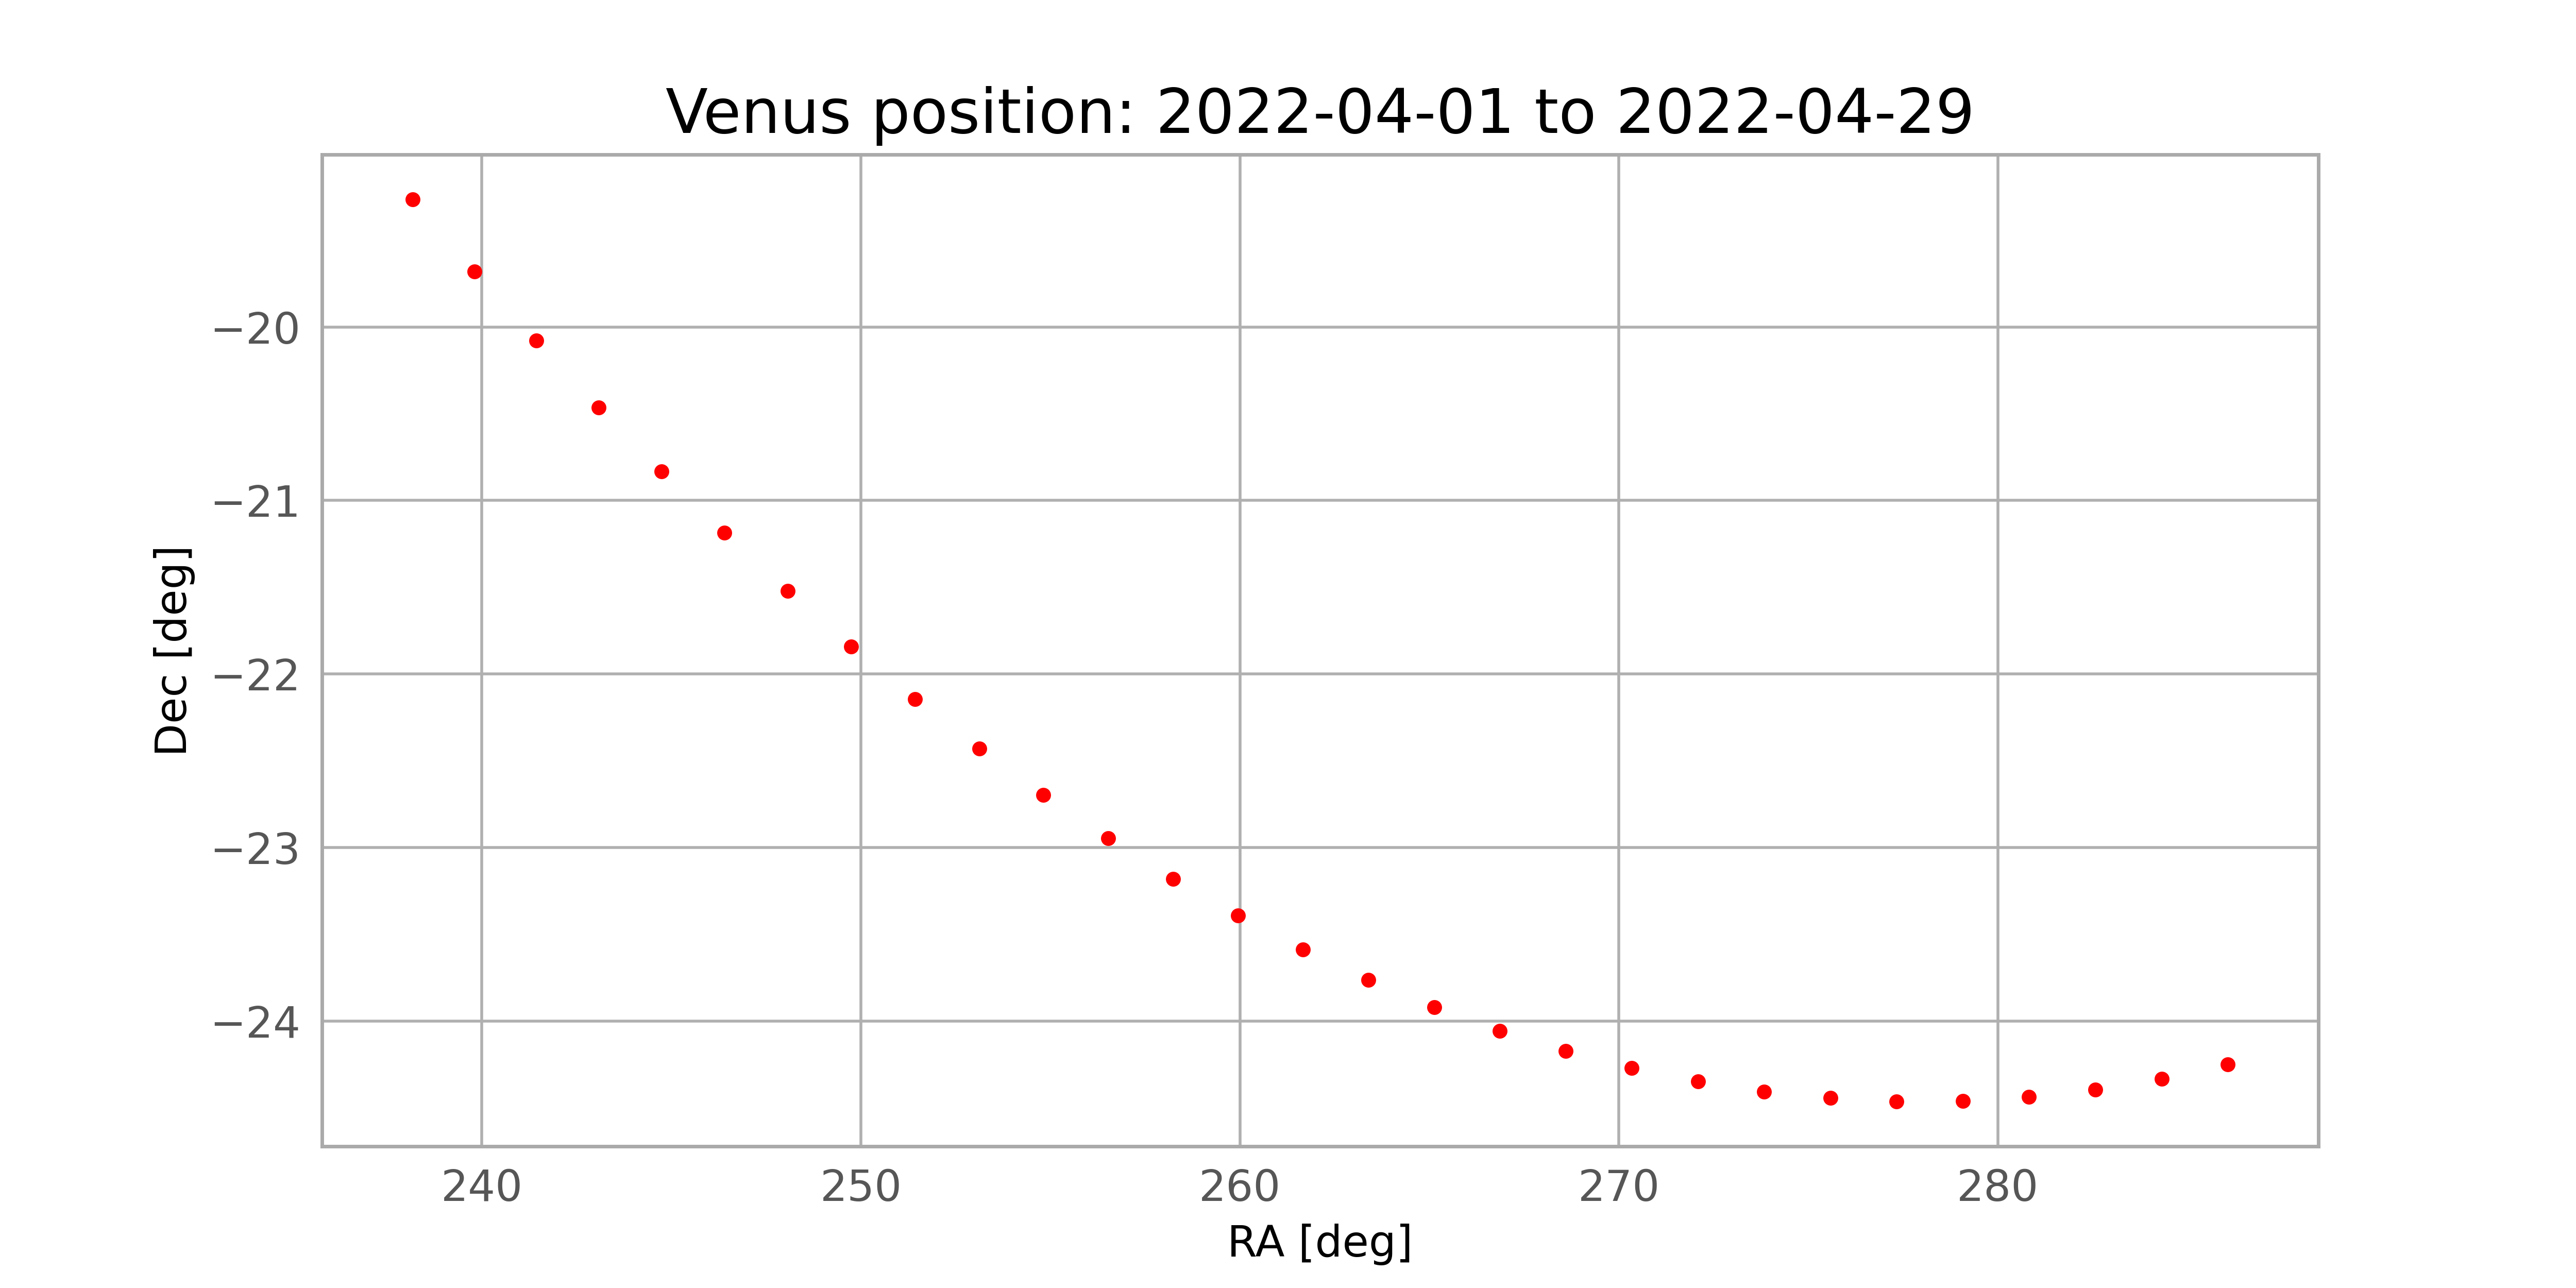
\includegraphics[width=\linewidth]{report/Figures/methods/Venus_position.png}
	\caption{Bovine pulmonary artery endothelial cells in culture. Blue: nuclei; red: mitochondria; green: microfilaments. Computer generated image from a 3D model based on a confocal laser scanning microscopy using fluorescent marker dyes. Source: Heiti Paves, \href{https://commons.wikimedia.org/wiki/File:Fibroblastid.jpg}{https://commons.wikimedia.org/wiki/File:Fibroblastid.jpg}.}
	\label{fig:bpartery}
\end{figure*}

%------------------------------------------------

\section{Conclusion}

In the soft X-ray domain explored by Chandra, Venus was a clear source. In a harder domain (3 keV - 10 keV), this is less obvious with the data presented here. Many differences exist between both analyses, physical and data wise. First of all, Venus doesn't have strong fluorescent scattering in a > 3 keV energy range because these fluorescence mainly concern heavier elements that are only present in the Venusian atmosphere as traces\footnote{See \url{https://physics.nist.gov/PhysRefData/XrayTrans/Html/search.html} for a list of fluorescence scattering energies and \cite{Futaana2017SolarAtmosphere}}. Secondly, Venus was only serendipitously observed in the \textit{INTEGRAL} data and it moved in the image. The data was therefore by construction less quality as the one retrieved by the Chandra spacecraft although the observation conditions were almost as optimal given the orbital parameters. However, the average fluxes calculated were all positive at a high significance level which suggest that the observation was not unsuccessful although more analysis should be made to ascertain this statement. Probing these higher energies are also the occasion to explore different emission processes and thresholds should be computed. Indeed, charge exchange interactions between highly charged heavy solar wind ions and atmospheric neutrals is the dominant process for the X-ray emission of comets for which Venus is a giant version\cite{Futaana2017SolarAtmosphere}.

The concordance between the solar and venusian flux showed its limits of applicability because of the lack of information on potential events hitting Venus. The event direction locator using the HEK gives however a good idea of the high number of events hitting the magnetic field deprived planet every single day.

In conclusion, the study of solar system planets in harder X-ray energies presents an interesting avenue for exploration. The extensive data gathered by the \textit{INTEGRAL} satellite over the past 19 years shows promise for conducting further analysis in this field. By delving deeper into this research, we have the potential to gain valuable insights into the behaviour of our neighbouring planets. The available \textit{INTEGRAL} data offers a solid foundation for future studies and encourages us to continue pushing the boundaries of this analysis.


%----------------------------------------------------------------------------------------
%	 REFERENCES
%----------------------------------------------------------------------------------------
\nocite{*}
\printbibliography % Output the bibliography

%----------------------------------------------------------------------------------------

\end{document}
